\chapter{Estudo Experimental}
\label{chap:descricaodostestes}

Neste capítulo discutiremos os testes realizados para avaliar o desempenho do método proposto.
Apresentaremos os conjuntos de dados usados e suas características gerais. 
Os algoritmos utilizados internamente no metaclassificador, assim como os \textit{Benchmark} dos testes também serão mostrados.
Por fim, discutiremos os resultados obtidos ao longo dos diversos testes.

\section{O Framework Weka}

Neste trabalho utilizamos o Framework \textit{Weka} para construir o metaclassificador que implementa nosso método proposto. 
O \textit{Weka} é uma coleção de algoritmos de aprendizado para tarefas gerais de mineração de dados \cite{Hall}.
Ele contém ferramentas de preprocessamento, classificação, regressão, clusterização, etc.
Ele pode ser utilizado para aplicar os algoritmos aos dados por meio de sua interface gráfica ou pode ser chamado diretamente de um código Java.

\section{\textit{Benchmark} dos testes}

Para avaliar a performance do método proposto um \textit{benchmark} específico é empregado em cada teste.
Quando um algoritmo é utilizado internamente no metaclassificador, e.g. Árvore de Decisão, o resultado deste mesmo algoritmo sem o metaclassificador é usado como \textit{benchmark}.
Isso é possível pois as classes que implementam estes algoritmos, que fazem parte do \textit{framework} Weka, são capazes de gerar uma distribuição de probabilidades de classes como saída.
A lista de saída que servirá como \textit{benchmark} do teste é então montada a partir desta distribuição de probabilidades.
Isto é, as classes são colocadas na lista na ordem decrescente de probabilidade.
Por exemplo, caso tenhamos as classes A, B, C e D com probabilidades 0.2, 0.25, 0.1 e 0.45 respectivamente, a lista de saída será D, B, A e C.

\section{As métricas de \textit{k-Acurácia}}

Recorde o caso da rede \textit{R} com \textit{n} nodos que podem apresentar falhas.
Imagine que sempre que a rede apresenta uma falha precisamos enviar uma ou mais equipes à nodos diferentes no intuito de corrigir o problema rapidamente.
No pior caso, sem qualquer indicio de onde a falha ocorreu, enviaremos \textit{n} equipes.
Porém, se por exemplo estivermos na dúvida entre apenas três nodos, saberemos que somente três equipes serão necessárias.

As métricas apresentadas nessa seção foram desenvolvidas para avaliar a performance dos modelos de acordo com esse cenário.
No caso da rede, precisamos de métricas que indiquem o grau de confiança que podemos ter ao enviar um certo número de equipes.
Como foi discutido, o metaclassificador recebe uma instância como entrada, neste caso medições sobre o estado de \textit{R} com ocorrência de falha.
Ele então retorna uma lista ordenada com as \textit{k} classes (nodos) mais prováveis.
De acordo com o problema proposto, a posição da classe verdadeira (nodo com falha) nesta lista é o fator mais importante.
Isto é, se a classe verdadeira aparece em uma das três primeiras posições da lista, este é o caso onde precisamos de apenas três equipes para efetuar o reparo.

Desta forma, a \textit{k-Acurácia} é na verdade um conjunto de métricas.
Elas variam de 1 até \textit{k}; i.e. \textit{1-Acurácia}, \textit{2-Acurácia} até \textit{k-Acurácia}; onde \textit{k} denota o tamanho da lista retornada.
Os valores das acurácias para uma dada instância dependem da posição da classe verdadeira na lista.
Se ela está na posição \textit{i}, onde $1 \leq \textit{i} \leq \textit{k}$, então as acurácias anteriores à \textit{i} tem o valor zero e o restante o valor um.
Com isso, a \textit{i-Acurácia} indica a certeza da classe verdadeira aparecer na lista até a posição \textit{i}.
Ou, sob a ótica do problema da rede, a confiança em reparar a falha se enviarmos esse mesmo número de equipes.

Observe na Figura \ref{fig:descricaodostestes01} diversos exemplos de listas e suas acurácias.
Para estes exemplos imagine que temos um conjunto de dados com cinco classes diferentes: A, B, C, D e E.
Considere também que a classe verdadeira em todos os casos ilustrados na Figura é A (em vermelho).
Cada linha do exemplo refere-se então a lista retornada para uma instância distinta e suas consequentes acurácias.

\begin{figure}[h!]
  \centering
  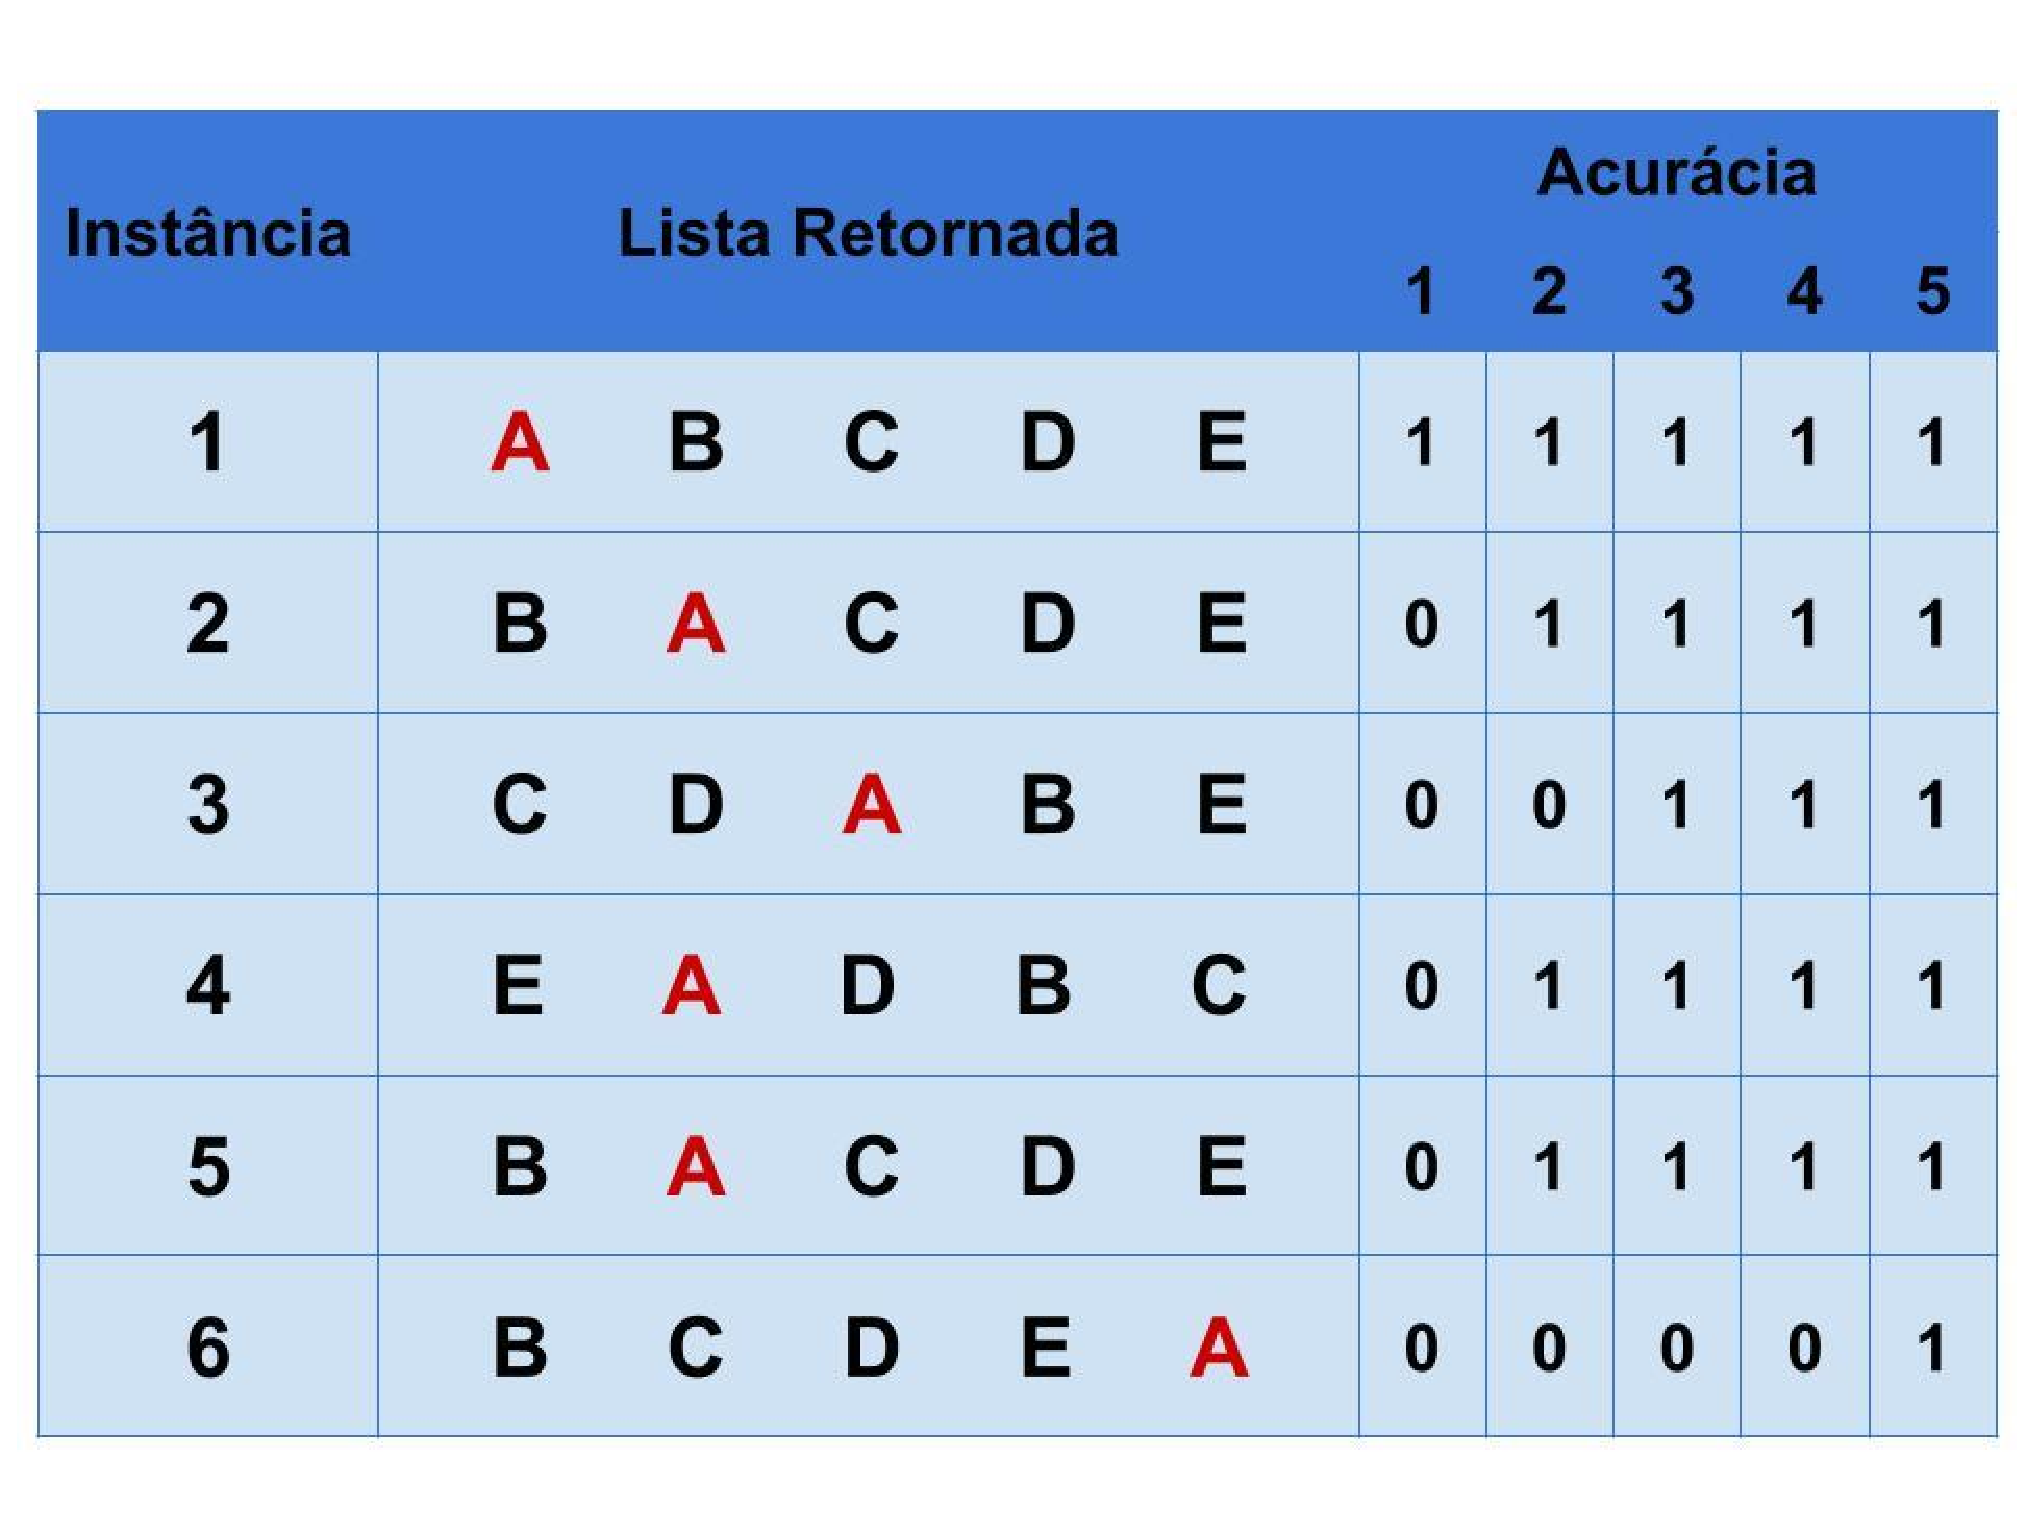
\includegraphics[width=100mm,scale=0.7]{images/descricaodostestes01.eps}
  \caption{Exemplos de listas e suas acurácias.}
  \label{fig:descricaodostestes01}
\end{figure}

Existe ainda uma diferença no cálculo da \textit{k-Acurácia} para o \textit{benchmark} dos testes.
Como a lista de \textit{benchmark} é construída a partir de uma distribuição de probabilidades, podem ocorrer empates.
Quando a probabilidade da classe verdadeira está empatada com a de uma ou mais classes, múltiplas listas poderiam ser criadas a partir desta distribuição.
Considere o caso onde temos as classes A, B e C com probabilidades 0.4, 0.4 e 0.2 respectivamente e a classe verdadeira é A.
Com essas probabilidades podemos ter as listas de saída (1) A, B e C ou (2) B, A e C.
No primeiro caso temos as acurácias de um a três iguais a um.
No segundo caso temos a \textit{1-Acurácia} igual a zero e o restante igual a um.
Entretanto, por ter acesso às probabilidades, a métrica divide os valores.
Teremos então \textit{1-Acurácia} igual 0.5, \textit{2-Acurácia} igual a 1 e \textit{3-Acurácia} igual a 1.

Note que todos os cálculos citados até agora são feitos por instância. 
Ao gerar listas de saída para múltiplas instâncias, os valores obtidos para cada acurácia são somados, formando um valor total por \textit{i-Acurácia}.
Este valor total é então dividido pelo número de instâncias que foram ranqueadas e multiplicado por cem.
Com isso os valores das acurácias apresentados neste trabalho estão na forma de percentuais.

Desta forma, podemos calcular os valores percentuais das acurácias ao longo de todos os exemplos da Figura \ref{fig:descricaodostestes01}.
Os valores são apresentados na tabela \ref{tab:valoresacuraciasexemplo}.

\begin{table}[h!]
  \begin{center}
    \begin{tabular}{cc}
      \hline
      \textbf{Acurácia} & \textbf{Valor Percentual} \\
      \hline

      1 & 16,67 \% \\
      2 & 66,67 \% \\
      3 & 83,33 \% \\
      4 & 83,33 \% \\
      5 & 100 \% \\

      \hline
    \end{tabular}
    \caption{Valores percentuais das acurácias do exemplo}
    \label{tab:valoresacuraciasexemplo}
  \end{center}
\end{table}

\section{As métricas k-Precision e k-Recall}

O \textit{k-Precision} e o \textit{k-Recall} são outros conjuntos de métricas que utilizamos na avaliação do método.
Estes são inspirados nas métricas \textit{Precision} e \textit{Recall}, largamente utilizadas em aprendizado de máquina.
Porém, da mesma forma como fizemos com as \textit{k-Acurácias}, adaptamos essas métricas para avaliar listas de classes de acordo com a posição da classe verdadeira.
Portanto, o \textit{k-Precision} e o \textit{k-Recall} também variam de 1 até \textit{k}; i.e. \textit{1-Precision}, \textit{2-Precision} até \textit{k-Precision}; onde \textit{k} denota o tamanho da lista retornada.

Como sabemos, os valores dessas métricas são calculados a partir da contabilização dos \textit{true positives (tp)}, \textit{false positives (fp)} e \textit{false negatives (fn)} (vide Capítulo \ref{chap:conceitosbasicos}).
Estes por sua vez dependem da posição da classe verdadeira na lista.
Se A é a classe verdadeira e ela aparece na posição \textit{i} da lista, onde $1 \leq \textit{i} \leq \textit{k}$, então as posições anteriores à \textit{i} contam como $fn_A$ e restante como $tp_A$.
Além disso, para cada posição anterior à \textit{i} também é contado um fp para a classe que foi prevista erradamente no lugar de A.

Observe na Figura \ref{fig:descricaodostestes02} o mesmo exemplo anterior agora com a contagem de tp, fn e fp para cada classe.
Recorde que no exemplo temos um conjunto de dados com as classes A, B, C, D e E, sendo A (em vermelho) a classe verdadeira em todos os exemplos.

\begin{figure}[h!]
  \centering
  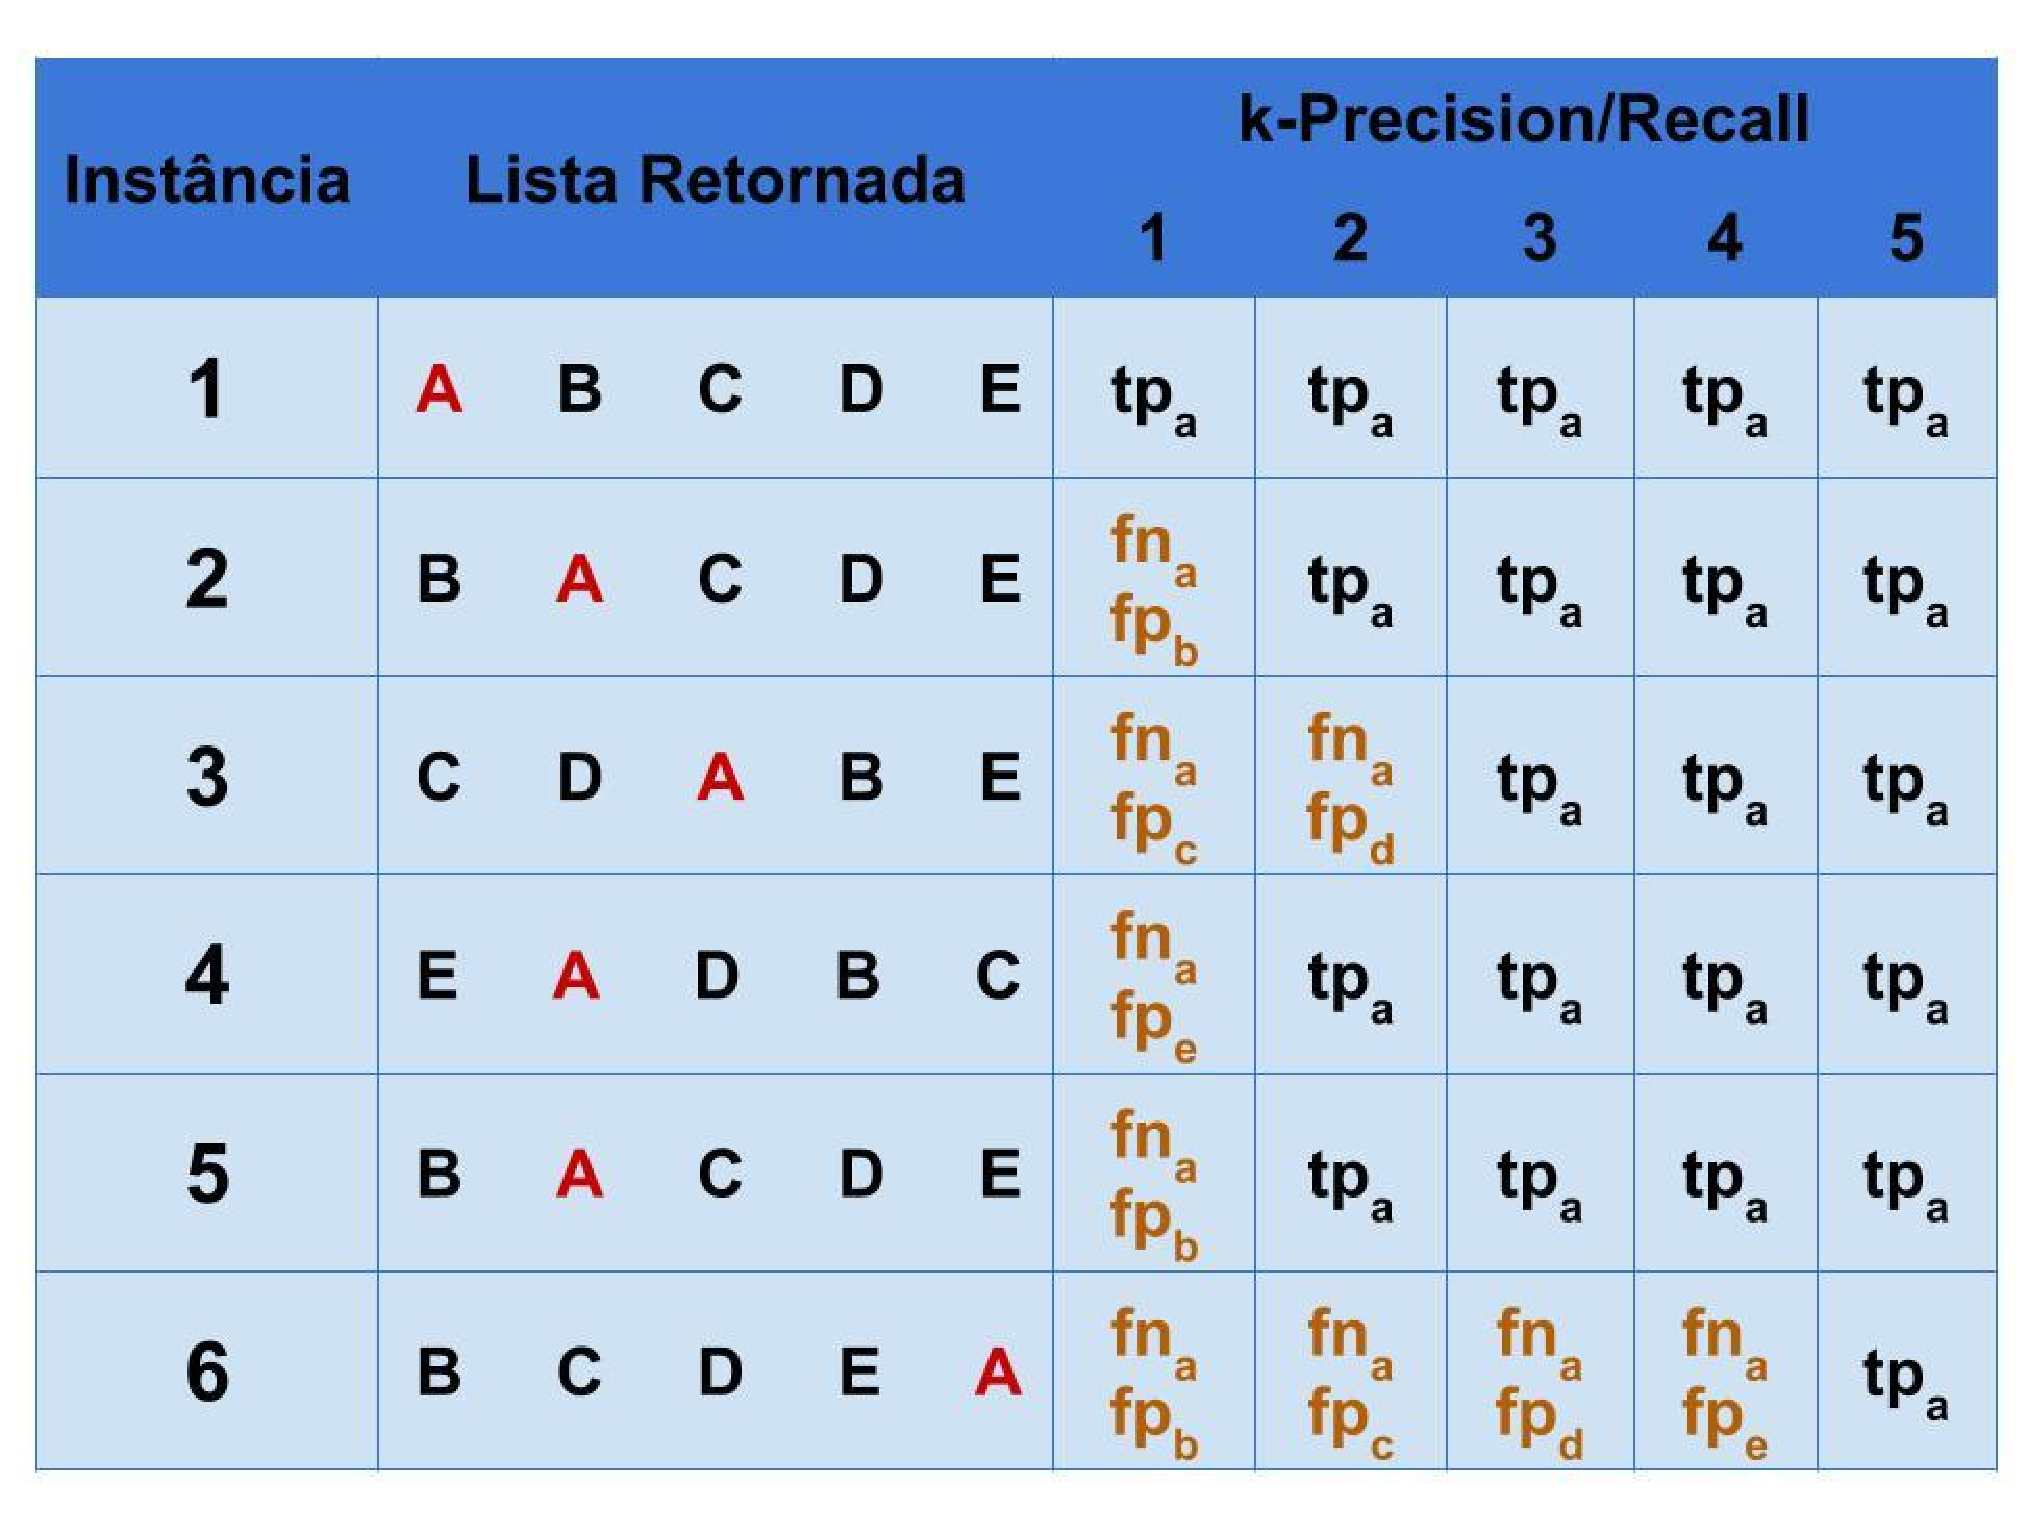
\includegraphics[width=120mm,scale=0.8]{images/descricaodostestes02.eps}
  \caption{Exemplos de listas e suas contagens de tp, fn e fp.}
  \label{fig:descricaodostestes02}
\end{figure}

Da mesma forma que fizemos para as \textit{k-Acurácias} o cálculo é feito de forma diferente para o \textit{benchmark} dos testes.
Lembre que quando a probabilidade da classe verdadeira está empatada com a de uma ou mais classes, múltiplas listas poderiam ser criadas a partir desta distribuição.
Retornemos ao exemplo da seção anterior, onde tínhamos as classes A, B e C com probabilidades 0.4, 0.4 e 0.2 respectivamente e onde a classe verdadeira é A.
Podemos ter as listas de saída (1) A, B e C ou (2) B, A e C.
No primeiro caso as posições de um a três contam como um $tp_A$.
No segundo caso a primeira posição conta um $fn_A$, um $fp_B$ e o restante das posições conta um $tp_A$.
Usando as probabilidades podemos contar de outra forma.
A primeira posição conta 0.5 $tp_A$, 0.5 $fn_A$ e 0.5 $fp_B$, visto que existe 50\% de chance de cada caso ocorrer.
O restante das posições conta simplesmente como um $tp_A$.

O cálculo do \textit{k-Precision} e do \textit{k-Recall} é feito de duas formas: \textit{Micro} e \textit{Média Ponderada}.
No primeiro caso somamos os \textit{true positives (tp)}, \textit{false positives (fp)} e \textit{false negatives (fn)} de todas as classes para cada \textit{i-Precision} e \textit{i-Recall}.
Depois aplicamos esses valores totais às fórmulas do \textit{Precision} e \textit{Recall}.
No segundo caso calculamos as métricas, usando as fórmulas, para cada classe a priori.
Depois tiramos uma média ponderada pela quantidade de cada classe no conjunto de dados.
Em ambos os casos os valores apresentados neste trabalho são convertidos para a forma de percentuais.

Desta forma, podemos calcular os valores percentuais do \textit{Micro Precision} e \textit{Micro Recall} ao longo de todos os exemplos da Figura \ref{fig:descricaodostestes02}.
Os valores são apresentados na tabela \ref{tab:valores_micro}.
Note que sempre teremos o mesmo valor para essas duas métricas pois a contagem total de \textit{false positives} e sempre igual a de \textit{false negatives}.

\begin{table}[h!]
  \begin{center}
    \begin{tabular}{ccc}
      \hline
      \textbf{k} & \textbf{Precision} & \textbf{Recall} \\
      \hline

      1 & 16,67 \% & 16,67 \% \\
      2 & 66,67 \% & 66,67 \% \\
      3 & 83,33 \% & 83,33 \% \\
      4 & 83,33 \% & 83,33 \% \\
      5 & 100 \% & 100 \% \\

      \hline
    \end{tabular}
    \caption{Valores percentuais do \textit{Micro Precision} e \textit{Micro Recall} do exemplo}
    \label{tab:valores_micro}
  \end{center}
\end{table}

\begin{figure}[h!]
  \centering
  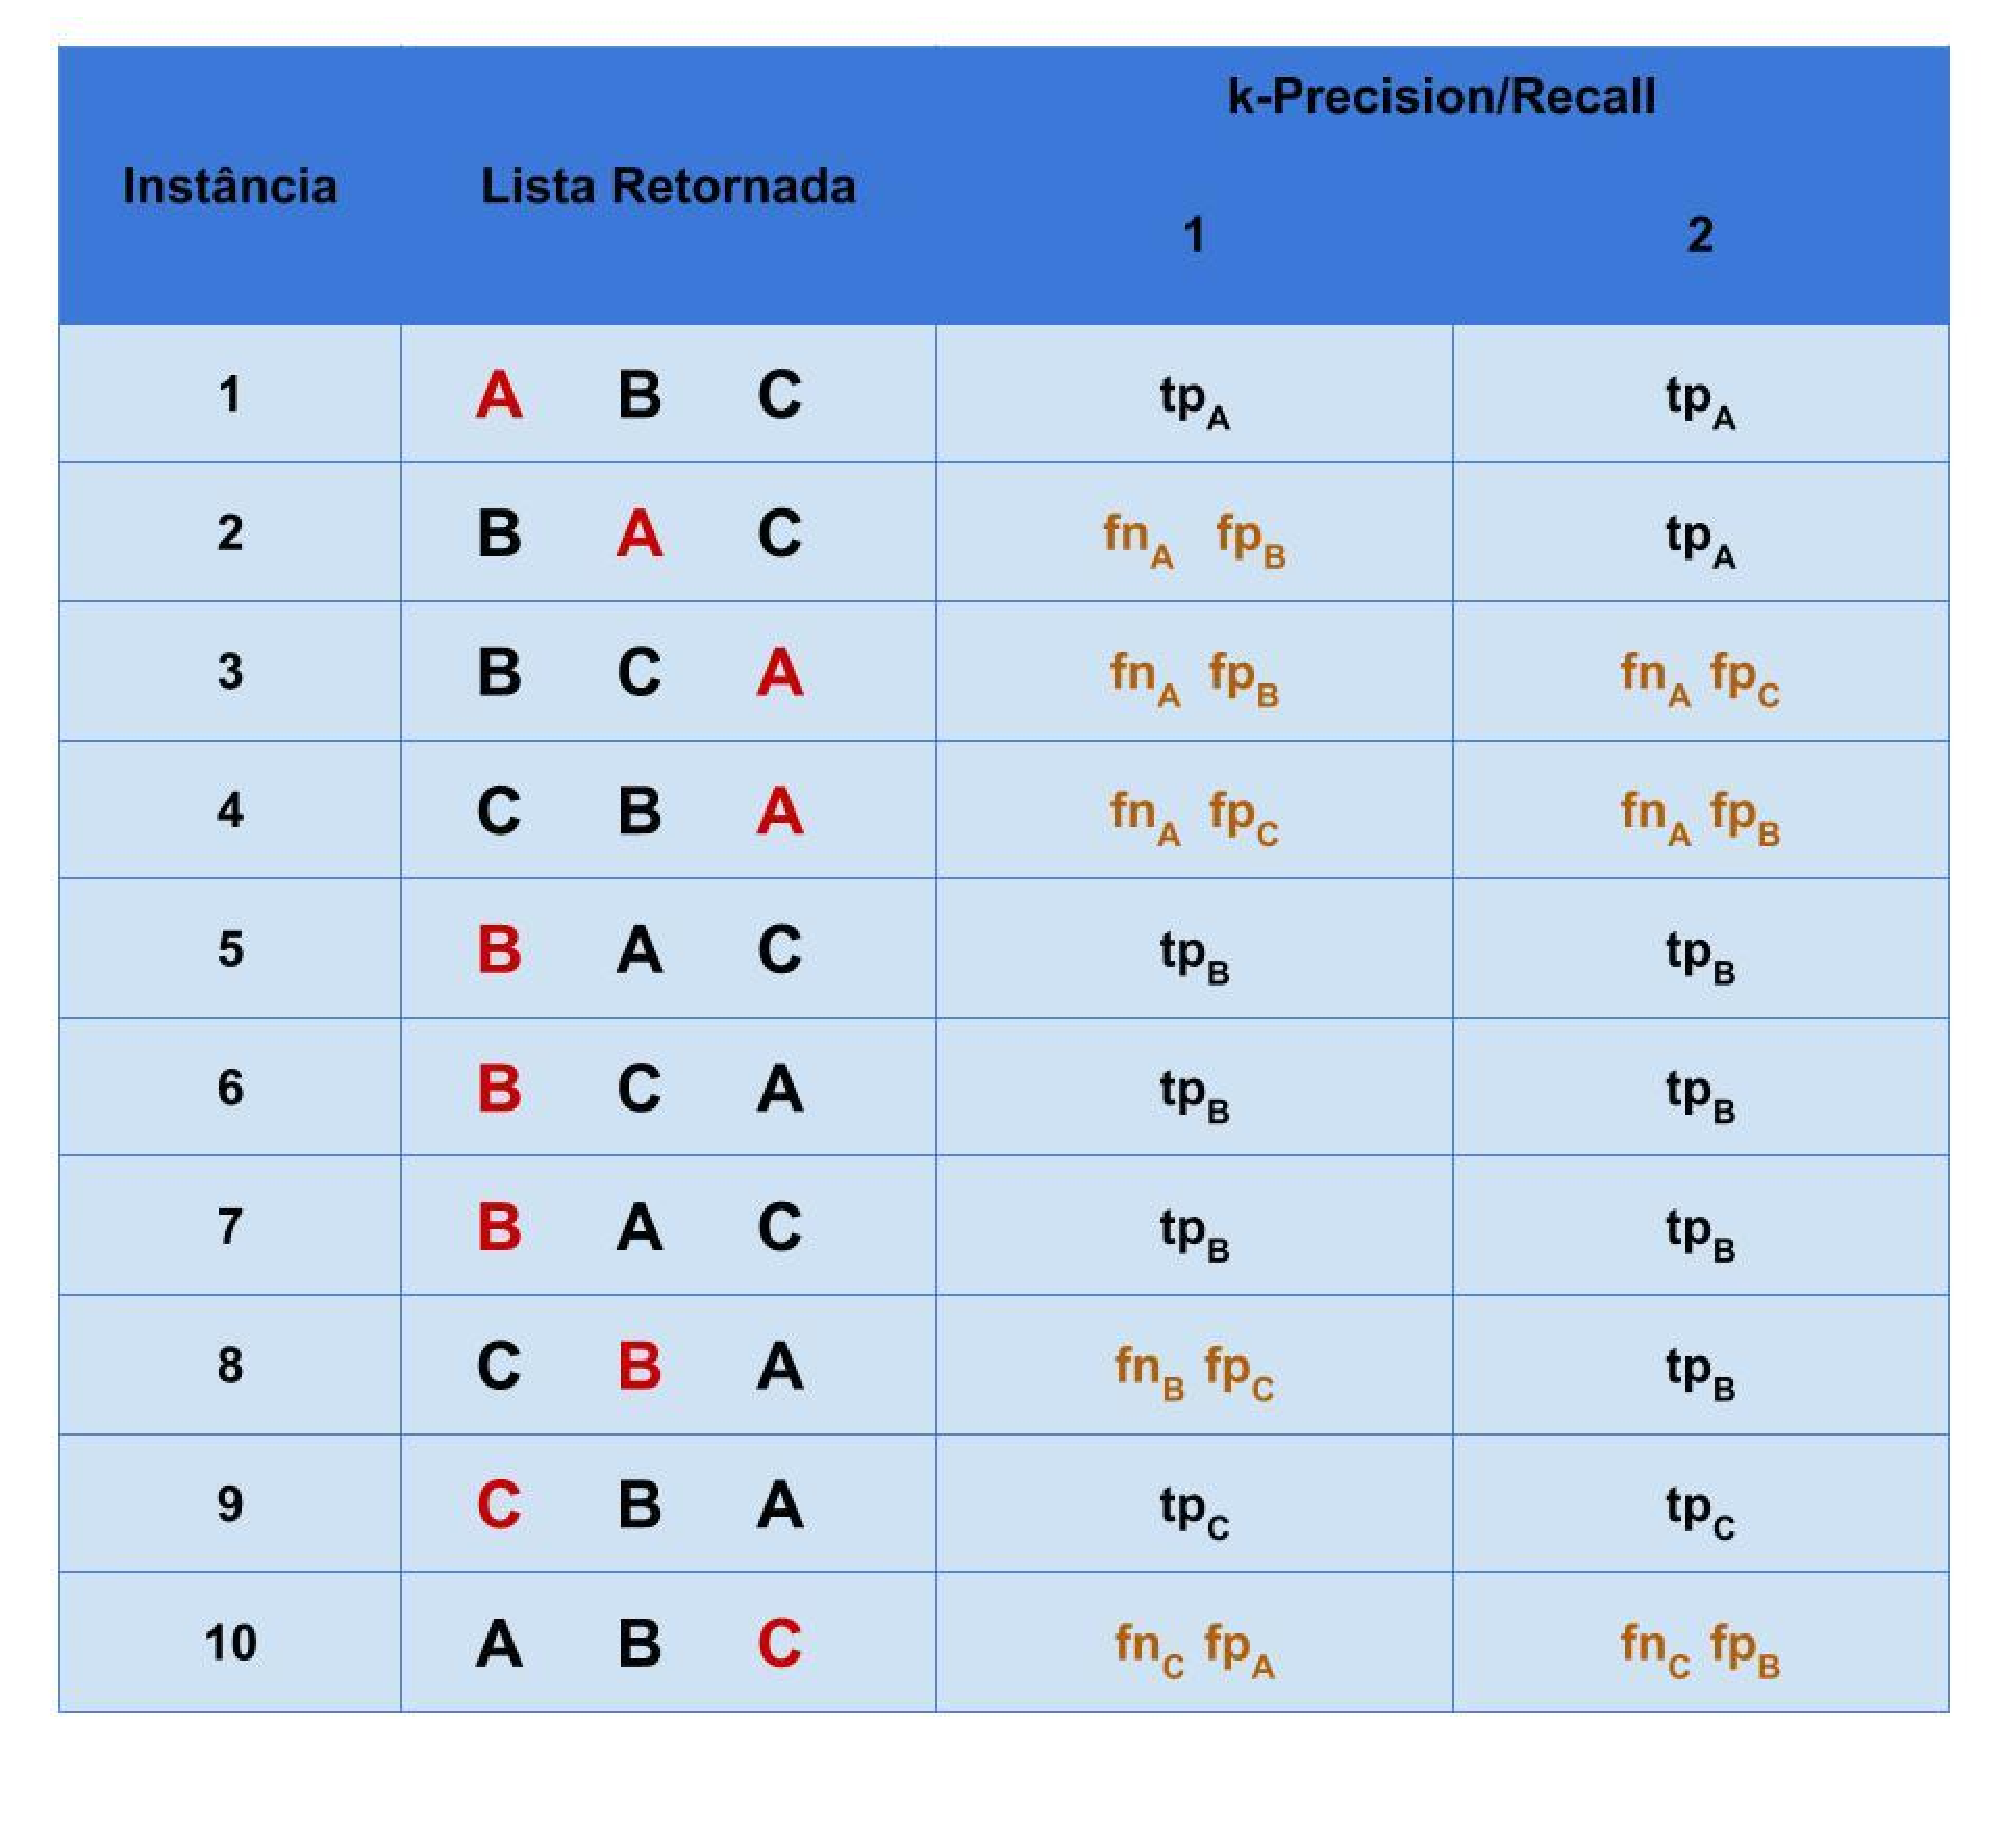
\includegraphics[width=120mm,scale=0.9]{images/descricaodostestes03.eps}
  \caption{Exemplos de listas com três classes e suas contagens de tp, fn e fp.}
  \label{fig:descricaodostestes03}
\end{figure}

Para entender o cálculo do \textit{Precision Ponderado} e do \textit{Recall Ponderado} mutilasse, considere outro exemplo onde temos apenas as classes A, B e C.
Este exemplo é apresentado na Figura \ref{fig:descricaodostestes03}, que mostra as dez listas retornadas e suas contagem de \textit{true positives}, \textit{false positives} e \textit{false negatives} para os níveis 1 e 2.

A partir disso podemos chegar às matrizes apresentadas na Tabela \ref{tab:confusao1} para as métricas de nível 1 e \ref{tab:confusao2} para as de nível 2.
Com os valores contabilizados em cada matriz é possível então calcular as métricas de nível 1 e 2 para cada classe, cujos resultados são apresentados na Tabela \ref{tab:valores_classes}.
Por fim, o valor final das métricas ponderadas é apresentado na Tabela \ref{tab:valores_pon}.

Para fazer esses cálculos utilizamos as fórmulas de \textit{Precision} e \textit{Recall} introduzidas no Capítulo \ref{chap:conceitosbasicos}.
Por exemplo, para chegar os valores do \textit{1-Precision Ponderado} da Tabela \ref{tab:valores_pon} devemos fazer os cálculos a seguir.
Considere que $N_A$, $N_B$ e $N_C$ são as quantidades de instancias das classes A, B e C respectivamente.

\begin{align*}
\text{1-Precision Ponderado} &= \frac{(\text{1-$Prec_A$} \times N_A)+(\text{1-$Prec_B$} \times N_B)+(\text{1-$Prec_C$} \times N_C)}{N_A+N_B+N_C} \\
&= \frac{(50\% \times 4)+(60\% \times 4)+(33,33\% \times 2)}{10} \\
&= 50,07\%
\end{align*}

\begin{table}[h!]
  \begin{center}
    \begin{tabular}{cccc}
      \hline
         & \textbf{Real: A} & \textbf{Real: B} & \textbf{Real: C} \\
      \hline

      Previsto: A & 1 & 0 & 1\\
      Previsto: B & 2 & 3 & 0\\
      Previsto: C & 1 & 1 & 1\\

      \hline
    \end{tabular}
    \caption{Contabilização dos valores para métricas ponderadas de nível 1}
    \label{tab:confusao1}
  \end{center}
\end{table}

\begin{table}[h!]
  \begin{center}
    \begin{tabular}{cccc}
      \hline
         & \textbf{Real: A} & \textbf{Real: B} & \textbf{Real: C} \\
      \hline

      Previsto: A & 2 & 0 & 0\\
      Previsto: B & 1 & 4 & 1\\
      Previsto: C & 1 & 0 & 1\\

      \hline
    \end{tabular}
    \caption{Contabilização dos valores para métricas ponderadas de nível 1}
    \label{tab:confusao2}
  \end{center}
\end{table}

\begin{table}[h!]
  \begin{center}
    \begin{tabular}{cccc}
      \hline
       Métrica  & \textbf{Classe A} & \textbf{Classe B} & \textbf{Classe C} \\
      \hline

      \textbf{1-Precision} & 50\% & 60\% & 33,33\% \\
      \textbf{2-Precision} & 100\% & 66,67\% & 50\% \\
      \textbf{1-Recall} & 25\% & 75\% & 50\% \\
      \textbf{2-Recall} & 50\% & 100\% & 50\% \\
      
      \hline
    \end{tabular}
    \caption{Contabilização dos valores métricas ponderadas de nível 1}
    \label{tab:valores_classes}
  \end{center}
\end{table}

\begin{table}[h!]
  \begin{center}
    \begin{tabular}{ccc}
      \hline
      \textbf{k} & \textbf{Precision} & \textbf{Recall} \\
      \hline

      1 & 50,07 \% & 50 \% \\
      2 & 76,67 \% & 70 \% \\

      \hline
    \end{tabular}
    \caption{Valores percentuais do \textit{Precision Ponderado} e \textit{Recall Ponderado} do exemplo}
    \label{tab:valores_pon}
  \end{center}
\end{table}

\section{Resultados dos Testes}

Todos os testes realizados neste capítulo foram realizados com validação cruzada com partição em dez grupos.
Novamente, os componentes do \textit{framework} Weka foram utilizados para realizar as validações.
Além disso, ao executar o programa 10 GB de memória são reservados para o \textit{heap} da Máquina Virtual Java com o comando \textit{java -Xmx10g}.

Todos os testes foram executados em máquinas virtuais no ambiente \textit{Google Cloud Platform}. 
Estas máquinas tinham a seguinte configuração: sistema operacional Linux Ubuntu 14.04, duas unidades de processamento (vCPU) e 13 GB de memória RAM.

Na Tabela \ref{tab:algoritmostestes} são apresentadas as configurações de algoritmos usados nos testes. Todas as classes utilizadas são do pacote \textit{weka.classifiers}.

\begin{table}[h!]
  \begin{center}
    \begin{tabular}{ccc}
      \hline
      \textbf{Algoritmo} & \textbf{Classe Weka} & \textbf{Opções} \\
      \hline

      Árvore de Decisão & trees.J48 & padrão \\
      Naive Bayes & bayes.NaiveBayes & padrão \\
      Support Vector Machine (SVM) & functions.SMO & padrão \\
      Random Forest & trees.RandomForest & padrão \\
      k vizinhos mais próximos (KNN) & lazy.IBk & K = 5, 7 e 9 \\

      \hline
    \end{tabular}
    \caption{Configurações dos algoritmos}
    \label{tab:algoritmostestes}
  \end{center}
\end{table}

Na Tabela \ref{tab:datasets} são apresentados as características gerais dos conjuntos de dados utilizados nos testes.
A maioria dos conjuntos de dados foi retirado do repositório \textit{UCI Machine Learning Repository}, disponível na internet no endereço http://archive.ics.uci.edu/ml/.
Além disso, em alguns casos o conjunto de dados foi preprocessado e reduzido para facilitar a realização dos diversos testes.
A exceção é o conjunto de dados Data-Zero, este não foi retirado do mesmo repositório.
O conjunto de dados Data-Zero representa a ocorrência de falhas em uma rede com diversos nodos.
Seu atributo classe denota em qual nodo a falha ocorreu.

\begin{table}[h!]
  \begin{center}
    \begin{tabular}{cccc}
      \hline
      \textbf{Conjunto de Dados} & \textbf{Instâncias} & \textbf{Atributos} & \textbf{Valores de Classe} \\
      \hline

      Iris & 150 & 5 & 3 \\
      Wine & 178 & 14 & 3 \\ 
      Glass & 214 & 10 & 7 \\
      Balance-Scale & 625 & 5 & 3 \\
      Segment-Challenge & 1500 & 20 & 7 \\
      Car & 1728 & 7 & 4 \\
      Data-Zero & 2846 & 202 & 42 \\
      Nursery & 3330 & 9 & 5 \\
      Poker-Hand & 3712 & 11 & 10 \\      
      Covtype-01percent & 5810 & 55 & 7 \\

      \hline
    \end{tabular}
    \caption{Conjuntos de dados}
    \label{tab:datasets}
  \end{center}
\end{table}

\subsection{Análise dos Tempos de Execução}

A Tabela \ref{tab:tempostestes} ilustra os tempos médios de execução para o conjunto de dados \textit{segment-challenge}, com uma lista de saída com tamanho três e validação cruzada com partição em dez grupos.
Os resultados para os demais conjuntos de treino seguem a mesma tendência e podem ser vistos por completo no apêndice.

A coluna \textit{Configuração} indica como a lista de saída foi construída.
Isto é, o teste pode ter empregado o modelo gerado pelo \textit{classificador} diretamente para construir a lista ou uma versão do método proposto (\textit{estática} ou \textit{dinâmica}).
A coluna \textit{Treino} informa o tempo médio de treinamento do modelo e a coluna \textit{Teste} o tempo médio que o modelo levou para gerar as listas de saída para as instâncias.
Estes valores foram obtidos com a média aritmética de cada Tempo ao longo das iterações da validação cruzada.

Note que, para todos os casos, temos que o tempo total do classificador é menor que os tempos das versões do método proposto.
Este resultado já era esperado, visto que o método proposto precisa treinar diversos classificadores para construir a lista de saída.
Além disso, a versão estática apresentou tempos totais maiores que a dinâmica.
Isso ocorre pois a primeira precisa treinar todos os classificadores possíveis a partir do conjunto de treino, enquanto a segunda treina apenas aqueles que são efetivamente utilizados.
Lembre que a versão dinâmica treina o modelo ao mesmo tempo que classifica as instâncias, portanto não é possível separar os tempos de treino e teste.
Por fim, uma vez que ambas as versões do método incorrem o mesmo resultado, somente a versão dinâmica foi utilizada nos demais testes apresentados neste capítulo.

\begin{table}[h!]
  \begin{center}
    \resizebox{\textwidth}{!} {
    \begin{tabular}{ccccc}
      \hline
      \textbf{Algoritmo} & \textbf{Configuração} & \textbf{Treino (ms)} & \textbf{Teste (ms)} & \textbf{Total (ms)}\\
      \hline

      Árvore de Decisão & classificador & 91.85 & 7.89 & 99.74\\
      Árvore de Decisão & estática & 515.80 & 6.70 & 522.51\\
      Árvore de Decisão & dinâmica & - & 405.87 & 405.87\\
      Naive Bayes &  classificador & 11.42 & 38.26 & 49.68\\
      Naive Bayes &  estática & 99.01 & 40.43 & 139.44\\
      Naive Bayes &  dinâmica & - & 100.95 & 100.95\\
      SVM & classificador & 240.37 & 4.18 & 244.55\\
      SVM & estática & 1646.29 & 6.45 & 1652.74\\
      SVM & dinâmica & - & 1340.57 & 1340.57\\
      Random Forest &  classificador & 449.76 & 8.62 & 458.38\\
      Random Forest &  estática & 5686.47 & 14.43 & 5700.89\\
      Random Forest &  dinâmica & - & 3934.28 & 3934.28\\
      KNN 5 & classificador & 0.89 & 23.76 & 24.66\\
      KNN 5 & estática  & 90.49 & 111.69  & 202.19\\
      KNN 5 & dinâmica  & - & 101.84 & 101.84\\

      \hline
    \end{tabular}
    }
    \caption{Tempos médios de execução em milissegundos}
    \label{tab:tempostestes}
  \end{center}
\end{table}

\subsection{Análise das Acurácias}

A Tabela \ref{tab:acuracias} exibe os valores de acurácia médios para cada algoritmo. 
Estes valores foram obtidos com a média aritmética de cada acurácia ao longo de todos os conjuntos de dados testados.
Novamente, a coluna \textit{Configuração} indica a forma como a lista de saída foi gerada. 
O valor \textit{classificador} significa que nestes testes usamos a distribuição de probabilidades do classificador para gerar a lista de saída, ou seja, é o \textit{benchmark} daquele teste.
Já o valor \textit{metaclassificador} significa que o método proposto (versão dinâmica) foi utilizado.
No intuito de facilitar a comparação, apresentamos as acurácias 1, 2 e 3 do classificador e do metaclassificador sempre em linhas subsequentes.

Além disso, é possível observar de forma rápida na tabela \ref{tab:acuracias2} quantas vezes cada configuração obteve o melhor resultado em cada acurácia.
Note que a contagem da tabela \ref{tab:acuracias2} se refere aos testes individuais e não às médias, ou seja, um teste por combinação de algoritmo e conjunto de dados.


\begin{table}[h!]
  \begin{center}
    \resizebox{\textwidth}{!} {
    \begin{tabular}{ccccc}
      \hline
      \textbf{Algoritmo} & \textbf{Configuração} & \textbf{1-Acurácia} & \textbf{2-Acurácia} & \textbf{3-Acurácia}\\
      \hline

Árvore de Decisão	&	classificador	&	78.97	&	86.85	&	90.9	\\
Árvore de Decisão	&	metaclassificador	&	79.1	&	91.37	&	96.37	\\
NaiveBayes	&	classificador	&	71.7	&	85.44	&	93.68	\\
NaiveBayes	&	metaclassificador	&	71.7	&	85.36	&	93.64	\\
SVM	&	classificador	&	77.86	&	90.2	&	95.62	\\
SVM	&	metaclassificador	&	77.82	&	90.16	&	95.71	\\
RandomForest	&	classificador	&	84.24	&	93.74	&	97.75	\\
RandomForest	&	metaclassificador	&	84.28	&	93.21	&	97.67	\\
KNN 5	&	classificador	&	80.66	&	90.84	&	94.73	\\
KNN 5	&	metaclassificador	&	80.45	&	91.3	&	96.24	\\
KNN 7	&	classificador	&	80.17	&	90.97	&	95.3	\\
KNN 7	&	metaclassificador	&	79.92	&	91.28	&	96.18	\\
KNN 9	&	classificador	&	80.03	&	91.04	&	95.67	\\
KNN 9	&	metaclassificador	&	79.93	&	90.56	&	95.93	\\

      \hline
    \end{tabular}
    }
    \caption{Valores de acurácia médios por algoritmo}
    \label{tab:acuracias}
  \end{center}
\end{table}

\begin{table}[h!]
  \begin{center}
    \begin{tabular}{cccc}
      \hline
      \textbf{Ganhador} & \textbf{1-Acurácia} & \textbf{2-Acurácia} & \textbf{3-Acurácia}\\
      \hline

Classificador	&	20	&	18	&	16	\\
Metaclassificador	&	19	&	32	&	26	\\
Empate	&	31	&	20	&	28	\\

      \hline
    \end{tabular}
    \caption{Número de vezes que cada configuração ganhou}
    \label{tab:acuracias2}
  \end{center}
\end{table}

Observe na Tabela \ref{tab:acuracias} que os valores da \textit{1-Acurácia} são sempre muito similares para o classificador e o metaclassificador.
Este resultado é esperado pois o primeiro modelo interno do metaclassificador (aquele que foi treinado com todo o conjunto de treino) é sempre igual ao modelo que gera a distribuição de probabilidades para o \textit{benchmark}.
Como foi explicado, quando ocorre empate de probabilidades na construção desse \textit{benchmark}, a métrica \textit{k-Acurácia} distribui o valor total entre as posições empatadas.
Desta forma, as diferenças na \textit{1-Acurácia} observadas na Tabela \ref{tab:acuracias} são devidas ao tratamento diferente nestes casos de empate.

Ainda na Tabela \ref{tab:acuracias}, note que o metaclassificador destacou-se nos testes com o algoritmo Árvore de Decisão.
Ele teve cerca de 4,5\% de vantagem na \textit{2-Precision} e 5,5\% na \textit{3-Precision}.
Nos demais casos as diferenças nas acurácias foram muito pequenas, em alguns o classificador teve um resultado marginalmente melhor em outros o metaclassificador.

\subsection{Análise do \textit{Precision} e \textit{Recall}}

As Tabelas \ref{tab:prec_micro} e \ref{tab:prec_pon} exibem respectivamente os valores de \textit{Micro Precision} e \textit{Precision Ponderado} médios para cada algoritmo.
Estes valores foram gerados calculando-se a média aritmética de cada métrica ao longo de todos os conjuntos de dados testados.
Como anteriormente, a coluna \textit{Configuração} denota a forma como a lista de saída foi gerada. 
Nesta coluna o valor \textit{classificador} indica o \textit{benchmark} do teste enquanto o valor \textit{metaclassificador} o resultado do método proposto (versão dinâmica).
Note que, os \textit{Precisions} 1, 2 e 3 do classificador e do metaclassificador são apresentados em linhas subsequentes.

Como já era esperado, o \textit{Micro Recall} resultou nos mesmos valores que o \textit{Micro Precision}, exibidos na Tabela \ref{tab:prec_micro}.
Além disso, o \textit{Recall Ponderado} também resultou nesses mesmos valores.
Portanto não apresentaremos tabelas com valores de \textit{Recall}.

\begin{table}[h!]
  \begin{center}
    \resizebox{\textwidth}{!} {
    \begin{tabular}{ccccc}
      \hline
      \textbf{Algoritmo} & \textbf{Configuração} & \textbf{1-Precision} & \textbf{2-Precision} & \textbf{3-Precision}\\
      \hline

Árvore de Decisão	&	classificador	&	79.1	&	88.03	&	90.8	\\
Árvore de Decisão	&	metaclassificador	&	79.1	&	91.37	&	96.37	\\
NaiveBayes	&	classificador	&	71.7	&	85.44	&	93.68	\\
NaiveBayes	&	metaclassificador	&	71.7	&	85.36	&	93.64	\\
SVM	&	classificador	&	77.82	&	89.9	&	94.99	\\
SVM	&	metaclassificador	&	77.82	&	90.16	&	95.71	\\
RandomForest	&	classificador	&	84.28	&	93.44	&	97.53	\\
RandomForest	&	metaclassificador	&	84.28	&	93.21	&	97.67	\\
KNN 5	&	classificador	&	80.45	&	89.46	&	93.38	\\
KNN 5	&	metaclassificador	&	80.45	&	91.3	&	96.24	\\
KNN 7	&	classificador	&	79.92	&	89.92	&	94.01	\\
KNN 7	&	metaclassificador	&	79.92	&	91.28	&	96.18	\\
KNN 9	&	classificador	&	79.93	&	89.98	&	94.24	\\
KNN 9	&	metaclassificador	&	79.93	&	90.56	&	95.93	\\

      \hline
    \end{tabular}
    }
    \caption{Valores de \textit{Micro Precision} médios por algoritmo}
    \label{tab:prec_micro}
  \end{center}
\end{table}

\begin{table}[h!]
  \begin{center}
    \resizebox{\textwidth}{!} {
    \begin{tabular}{ccccc}
      \hline
      \textbf{Algoritmo} & \textbf{Configuração} & \textbf{1-Precision} & \textbf{2-Precision} & \textbf{3-Precision}\\
      \hline

Árvore de Decisão	&	classificador	&	78.68	&	89.98	&	93.3	\\
Árvore de Decisão	&	metaclassificador	&	78.68	&	90.74	&	96.27	\\
NaiveBayes	&	classificador	&	73	&	85.84	&	93.4	\\
NaiveBayes	&	metaclassificador	&	73	&	85.71	&	93.32	\\
SVM	&	classificador	&	75.99	&	87.3	&	93.26	\\
SVM	&	metaclassificador	&	75.99	&	87.61	&	93.97	\\
RandomForest	&	classificador	&	84.31	&	93.06	&	97.26	\\
RandomForest	&	metaclassificador	&	84.31	&	92.41	&	97.39	\\
KNN 5	&	classificador	&	79.55	&	89.48	&	94.01	\\
KNN 5	&	metaclassificador	&	79.55	&	90.9	&	96.05	\\
KNN 7	&	classificador	&	79.25	&	89.76	&	94.36	\\
KNN 7	&	metaclassificador	&	79.25	&	91	&	95.94	\\
KNN 9	&	classificador	&	78.99	&	89.77	&	94.54	\\
KNN 9	&	metaclassificador	&	78.99	&	89.9	&	95.65	\\

      \hline
    \end{tabular}
    }
    \caption{Valores de \textit{Precision Ponderado} médios por algoritmo}
    \label{tab:prec_pon}
  \end{center}
\end{table}

Além disso, é possível observar de forma rápida nas tabelas \ref{tab:count_micro} e \ref{tab:count_pon} quantas vezes cada configuração obteve o melhor resultado para cada métrica.
Lembre que as contagens nestas tabelas se referem aos testes individuais, i.e., um teste por combinação de algoritmo e conjunto de dados.

\begin{table}[h!]
  \begin{center}
    \begin{tabular}{cccc}
      \hline
      \textbf{Ganhador} & \textbf{1-Precision} & \textbf{2-Precision} & \textbf{3-Precision}\\
      \hline

Classificador	&	0	&	10	&	7	\\
Metaclassificador	&	0	&	40	&	43	\\
Empate	&	70	&	20	&	20	\\

      \hline
    \end{tabular}
    \caption{\textit{Micro Precision}: Número de vezes que cada configuração ganhou}
    \label{tab:count_micro}
  \end{center}
\end{table}

\begin{table}[h!]
  \begin{center}
    \begin{tabular}{cccc}
      \hline
      \textbf{Ganhador} & \textbf{1-Precision} & \textbf{2-Precision} & \textbf{3-Precision}\\
      \hline

Classificador	&	0	&	15	&	12	\\
Metaclassificador	&	0	&	37	&	39	\\
Empate	&	70	&	18	&	19	\\

      \hline
    \end{tabular}
    \caption{\textit{Precision Ponderado}: Número de vezes que cada configuração ganhou}
    \label{tab:count_pon}
  \end{center}
\end{table}

É possível observar nas Tabelas \ref{tab:prec_micro} e \ref{tab:prec_pon} que os valores da \textit{1-Precision} são muito próximos para o classificador (\textit{Benchmark}) e o metaclassificador.
Também é possível notar que, assim como ocorreu com as acurácias, o metaclassificador superou o \textit{benchmark} por margens maiores com o algoritmo Árvore de Decisão.
Ele teve cerca de 3,5\% de vantagem na \textit{2-Precision (Micro)}, 5,5\% na \textit{3-Precision (Micro)} e 3\% na \textit{3-Precision (Ponderada)}. 
Entretanto desta vez o algoritmo KNN também conseguiu se destacar na \textit{2-Precision} e \textit{3-Precision}, tanto nas versões \textit{Micro} quanto \textit{Ponderada}. 
Ele superou o \textit{benchmark} por margens superiores a 1\% nas \textit{2-Precision} e 2\% nas \textit{3-precision}.
Nos demais casos as diferenças entre classificador e metaclassificador foram muito pequenas (inferiores à 1\%).

\section{Testes com Dados Sintéticos}

Nos experimentos com conjuntos de dados retirados de bases públicas as métricas indicaram que o resultado do metaclassificador foi similar ao do \textit{benchmark}, superando este em alguns casos.
Entretanto, no intuito de entender melhor o comportamento do método proposto decidimos conduzir uma série de testes com dados sintéticos.
Estes dados foram construídos para emular características específicas nos dados, como por exemplo as quantidades de instâncias de cada classe balanceadas ou não.
Desta forma pudemos utilizar as métricas \textit{k-Acurácia}, \textit{k-Precision} e \textit{k-Recall} para entender como o método proposto responde à essas características dos conjuntos de dados.

\subsection{Descrição dos conjuntos de dados Sintéticos}
\label{sub:descsinteticos}

Todos os conjuntos de dados sintéticos que criamos são compostos por três classes: azul, vermelha e verde.
Para gerar os pontos dessas classes utilizamos distribuições normais bivariadas.
Veja a seção Motivação do Capítulo \ref{chap:metodoproposto} para mais detalhes sobre esse tipo de distribuição.
Sendo assim, cada instância tem dois atributos numéricos gerados aleatoriamente de acordo com a distribuição de sua classe.
Utilizamos a mesma matriz de covariâncias nas distribuições das três classes (apresentada abaixo).
Por outro lado, variamos as médias das distribuições e as quantidades de pontos de cada classe.

\begin{equation*}
\text{Matriz de Covariâncias} =\[\left( 
\begin{array}{cc}
	2,5  & 1,5 \\
	1,5 & 2,5 
\end{array} 
\right)\]
\end{equation*}

\begin{figure}
  \centering
  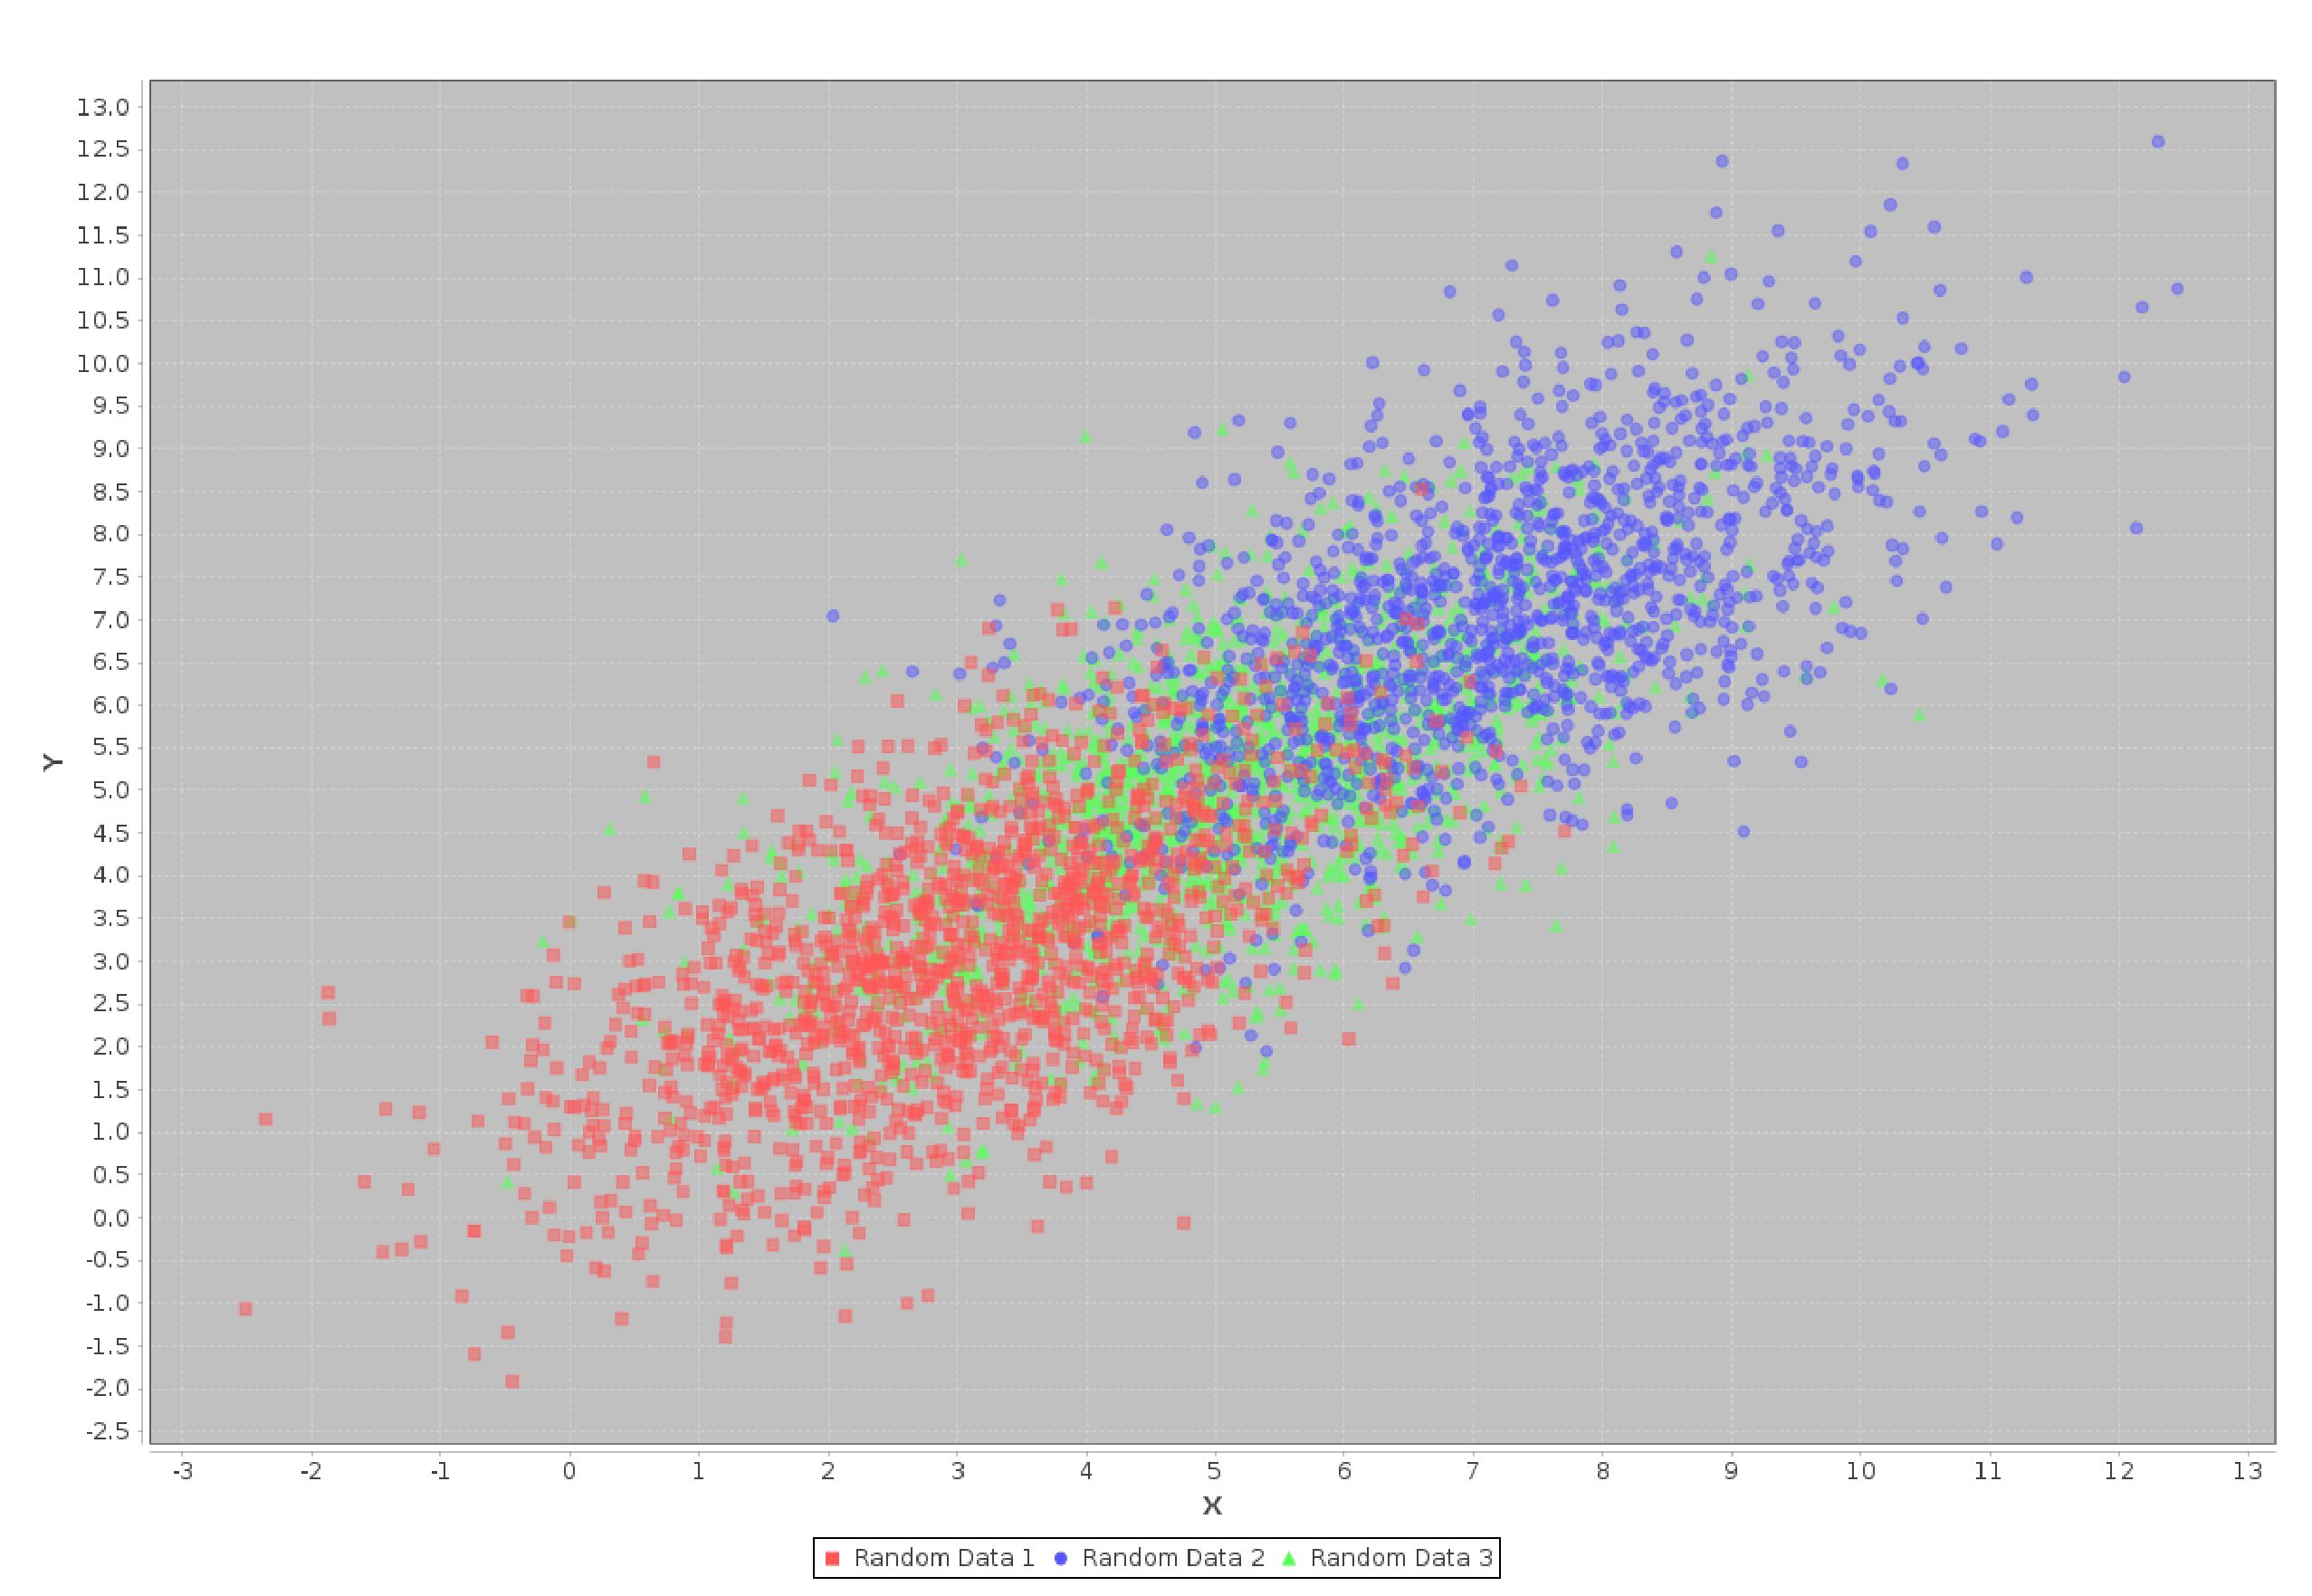
\includegraphics[width=120mm,scale=0.7]{images/dist1500-1500-5.eps}
  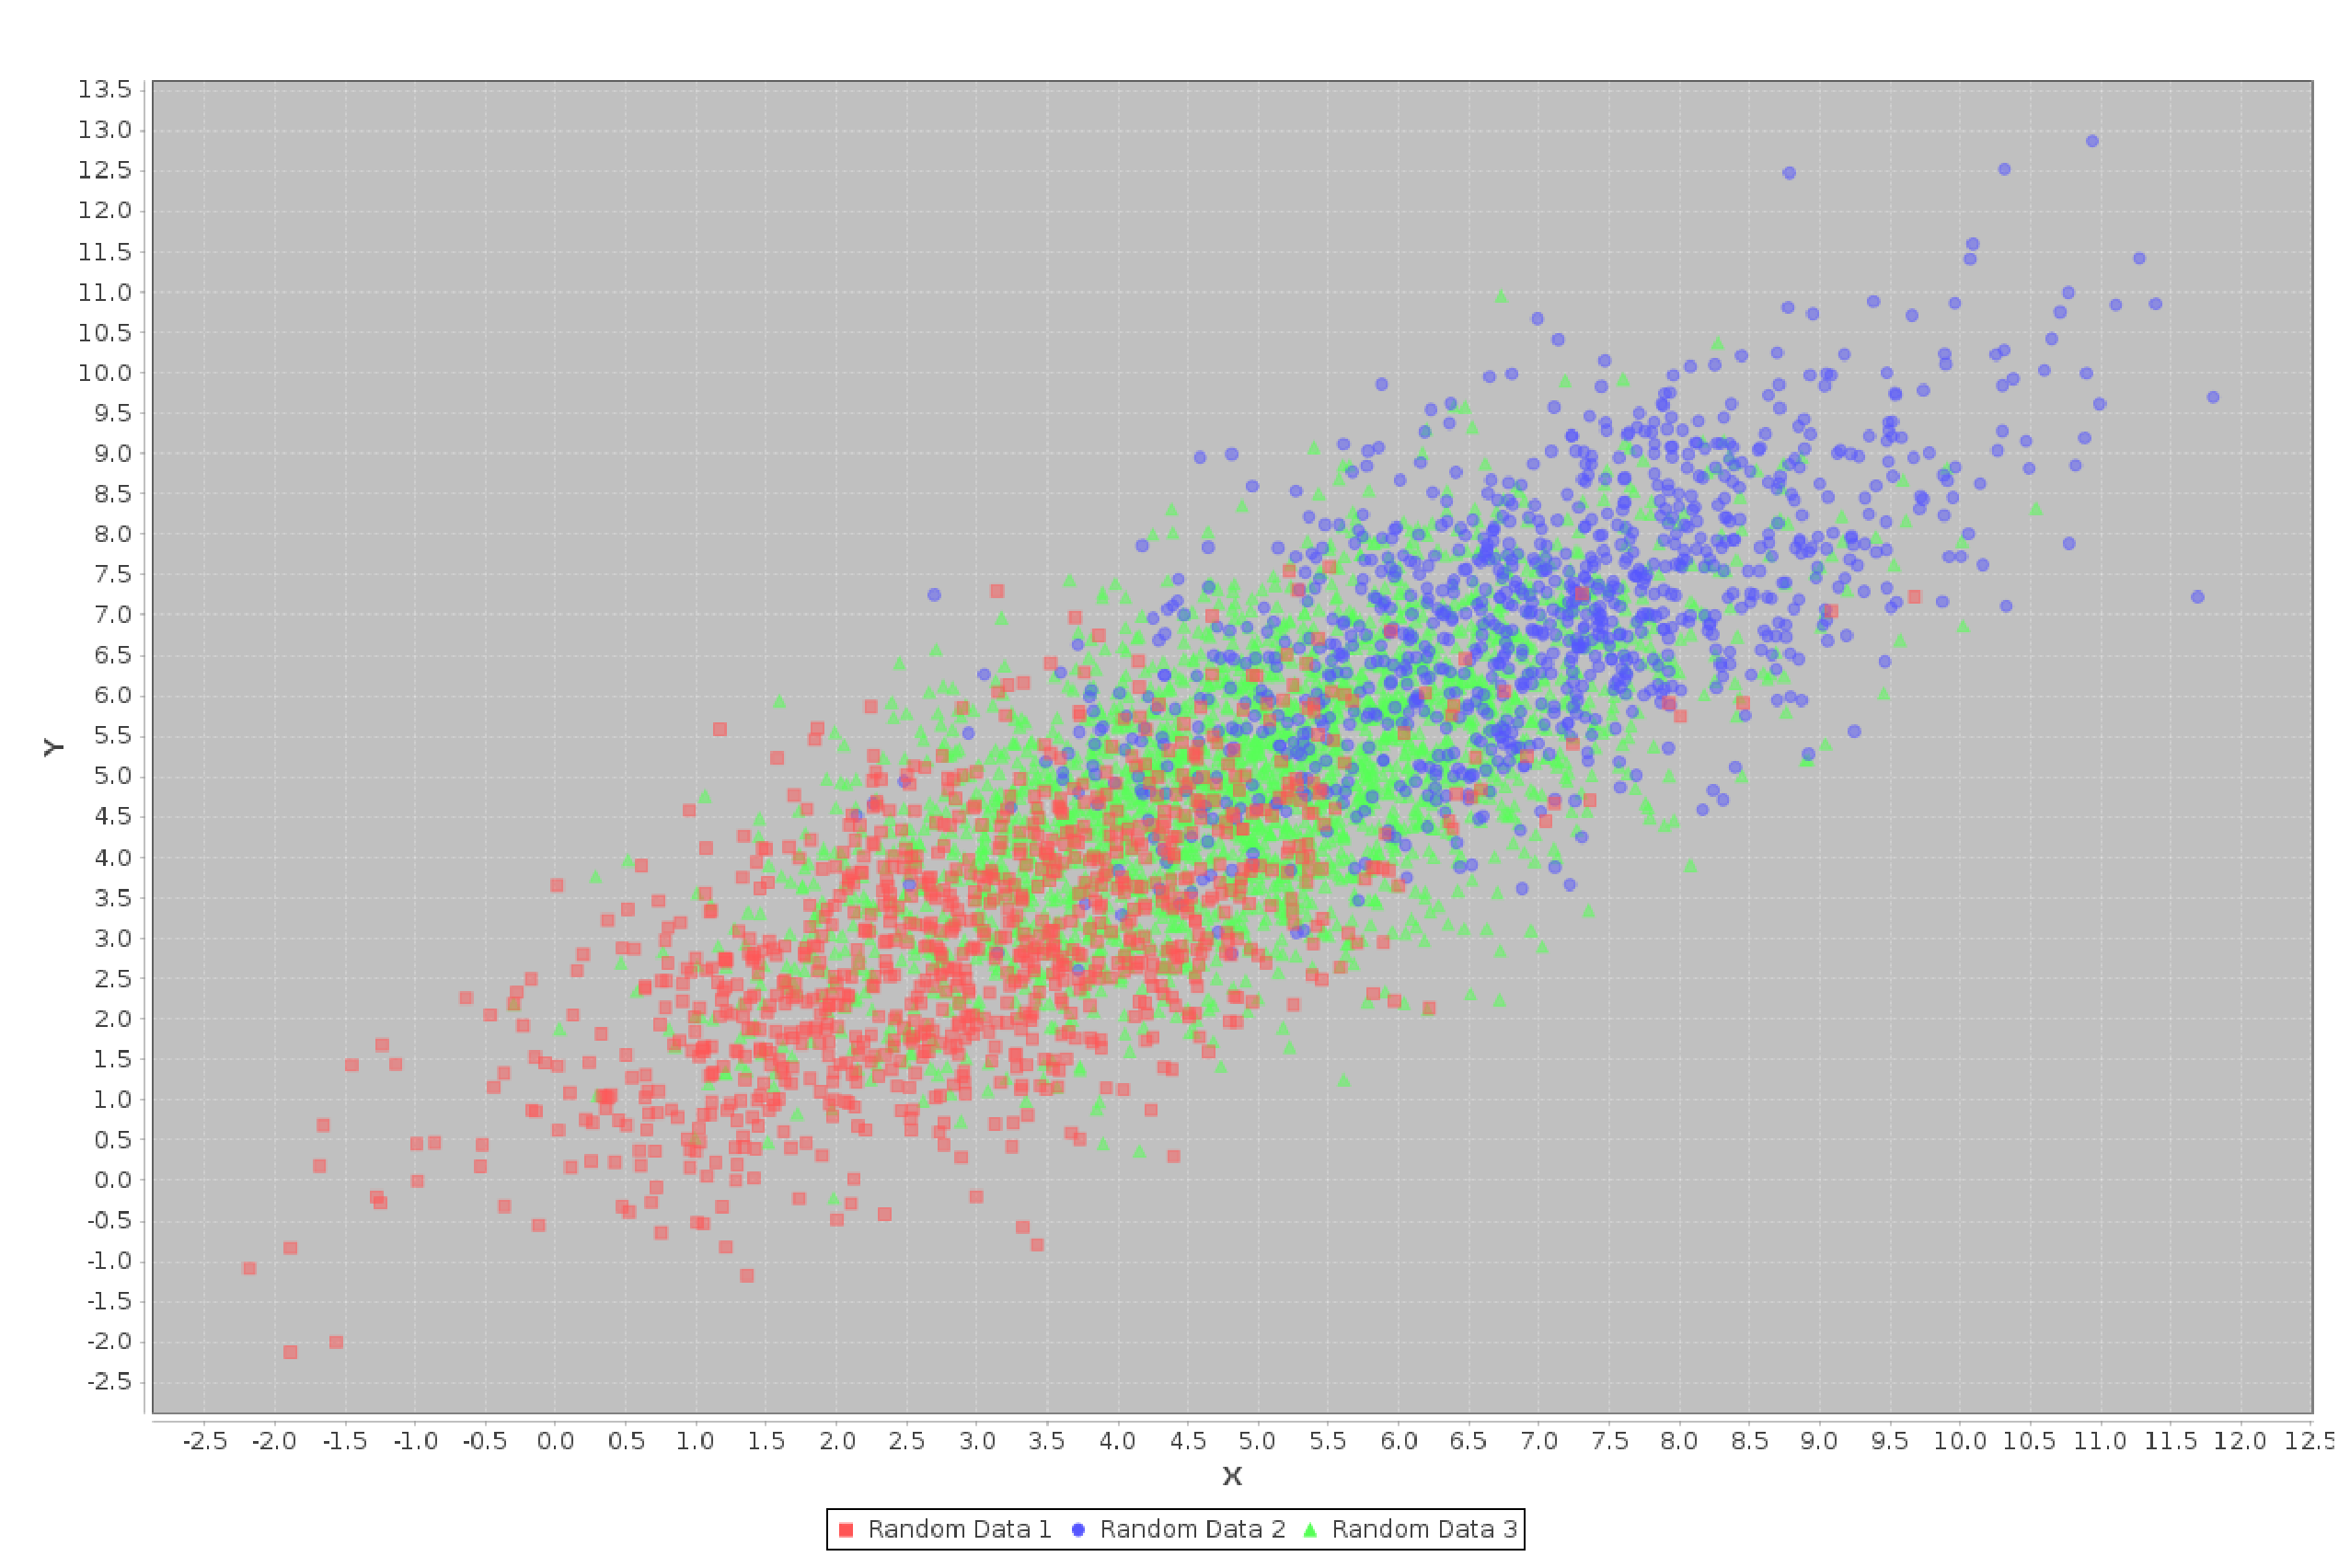
\includegraphics[width=120mm,scale=0.7]{images/dist1000-2500-5.eps}
  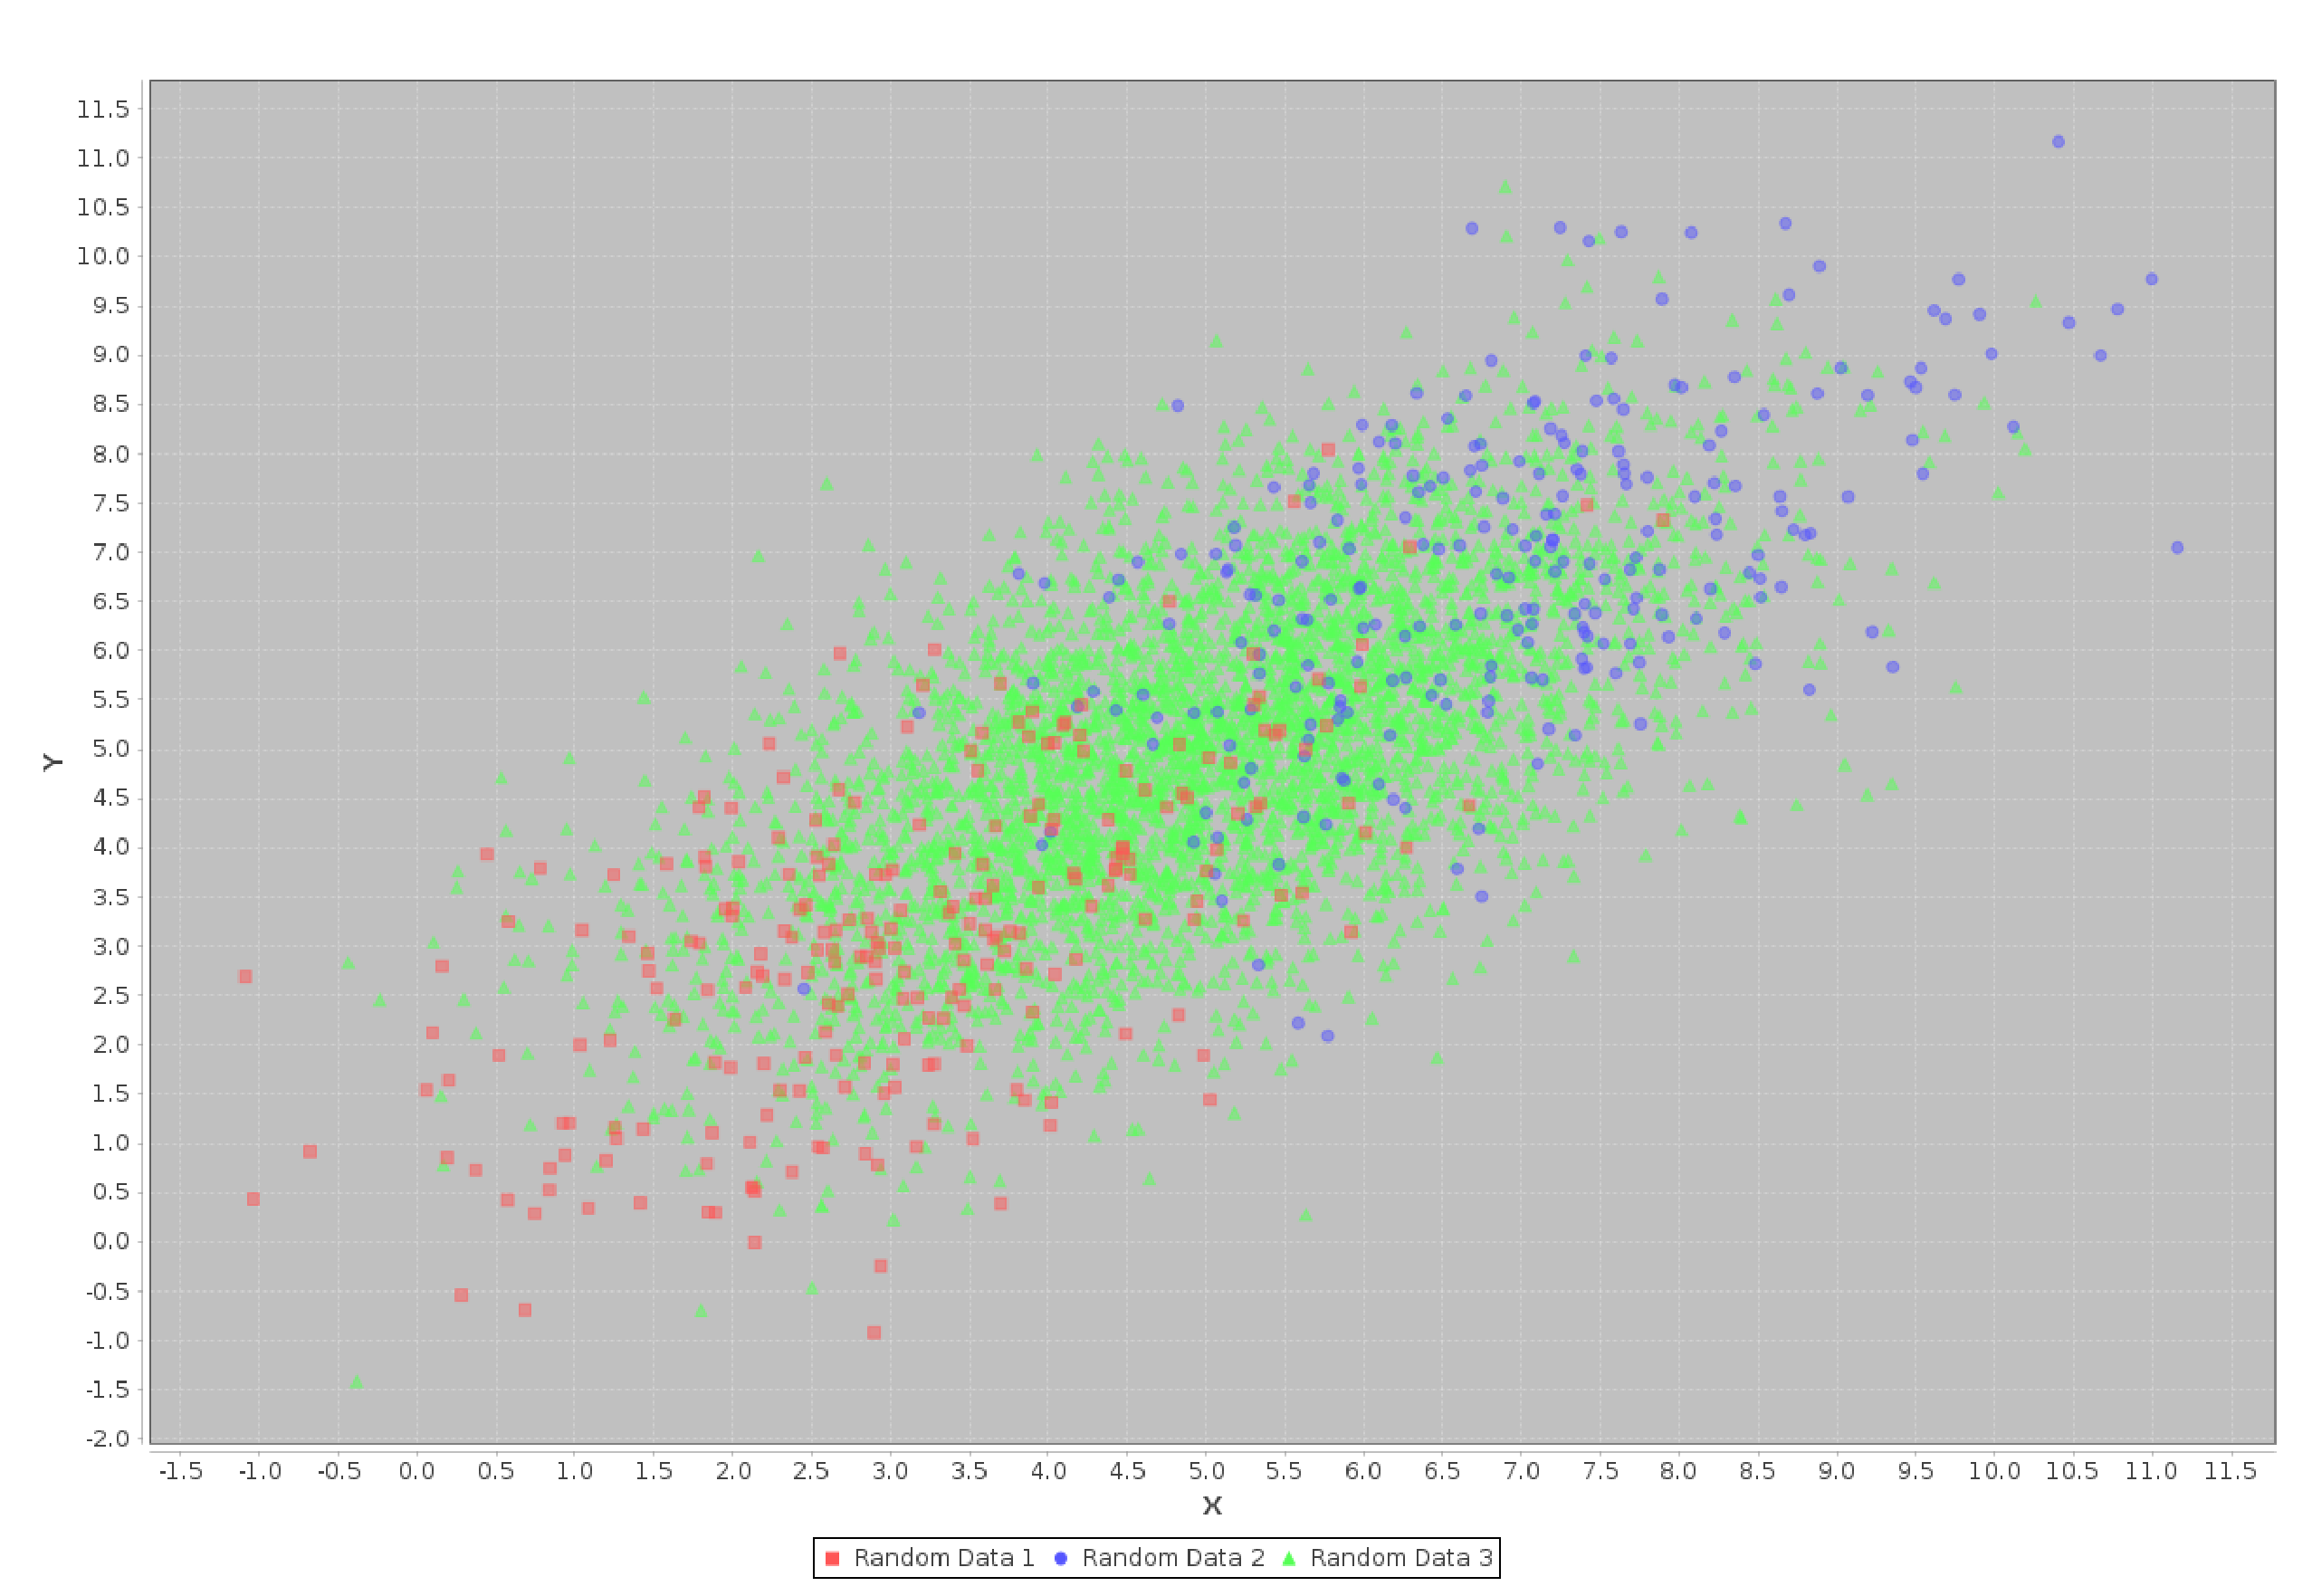
\includegraphics[width=120mm,scale=0.7]{images/dist250-4000-5.eps}
  \caption{Conjuntos de dados sintéticos com diferentes quantidades de instâncias de cada classe}
  \label{fig:dist_diferentes}
\end{figure}

Todos os conjuntos de dados criados tem 4500 pontos.
Entretanto versões com proporções diferentes de instâncias das classes foram criadas: \textit{balanceado}, \textit{normal} e \textit{desbalanceado}.
A tabela \ref{tab:dados_sinteticos} mostra as quantidades de instâncias de classes para as diferentes versões de dados.
A Figura \ref{fig:dist_diferentes} apresenta um conjunto de dados de cada versão.
Note que os três conjuntos de dados da Figura tem quantidades diferentes de instâncias de cada classe.
Todavia as médias das distribuições de cada classe nos diferentes conjuntos de dados são as mesmas.

\begin{table}[h!]
  \begin{center}
    \begin{tabular}{cccc}
      \hline
      \textbf{Conjunto de Dados} & \textbf{Verde} & \textbf{Azul} & \textbf{Vermelho}\\
      \hline

Balanceado (B)	&	 1500 & 1500 & 1500	\\
Normal (N)	&	 2500 & 1000 & 1000	\\
Desbalanceado (D)      & 4000 & 250 & 250	\\

      \hline
    \end{tabular}
    \caption{Versões de quantidades de instâncias de cada classe}
    \label{tab:dados_sinteticos}
  \end{center}
\end{table}

Além disso, os conjuntos de dados com a mesma distribuição também foram gerados em três versões diferentes.
Estas versões se diferenciam pelo posicionamento relativo das distribuições de classes: \textit{próxima}, \textit{adjacente} e \textit{distante}.
A Figura \ref{fig:dist_iguais} ilustra essas três versões para o conjunto de dados \textit{desbalanceado}.
Note que na versão \textit{próxima} a média da classe dominante (verde) está entre as médias das outras duas classes.
Nas versões \textit{adjacente} e \textit{distante} a média da classe dominante é afastada sucessivamente das outras duas classes.

\begin{figure}
  \centering
  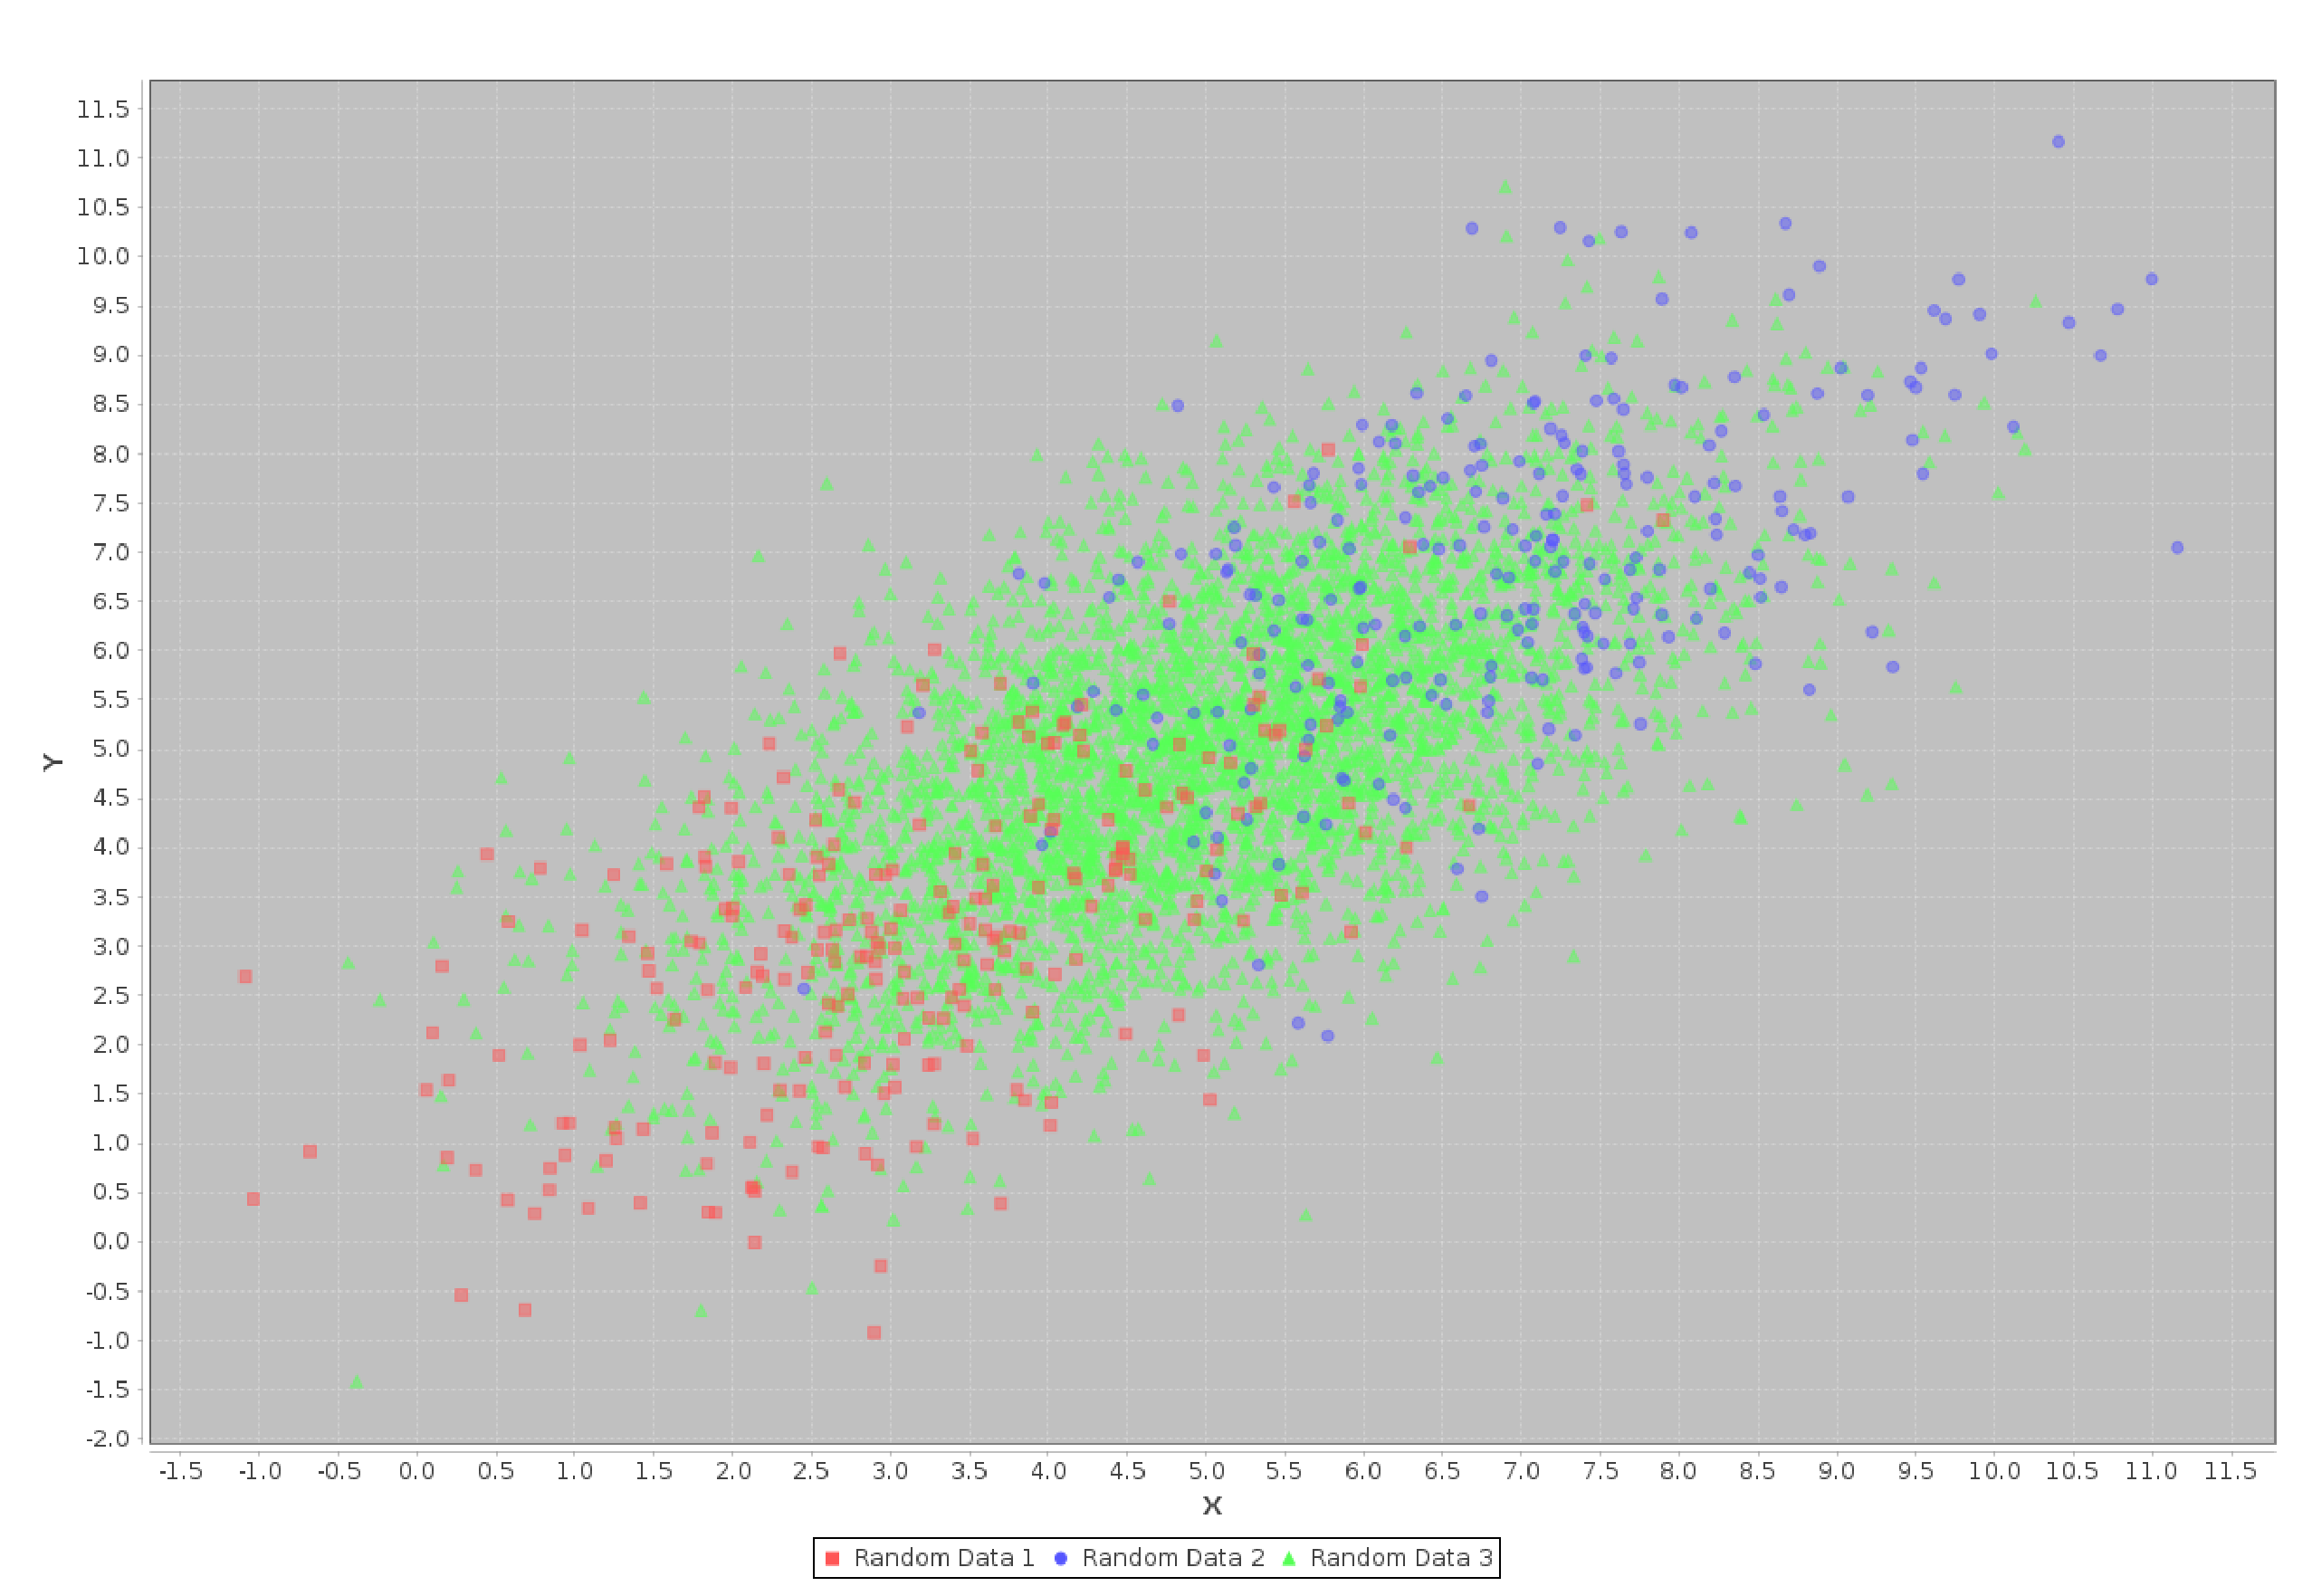
\includegraphics[width=120mm,scale=0.7]{images/dist250-4000-5.eps}
  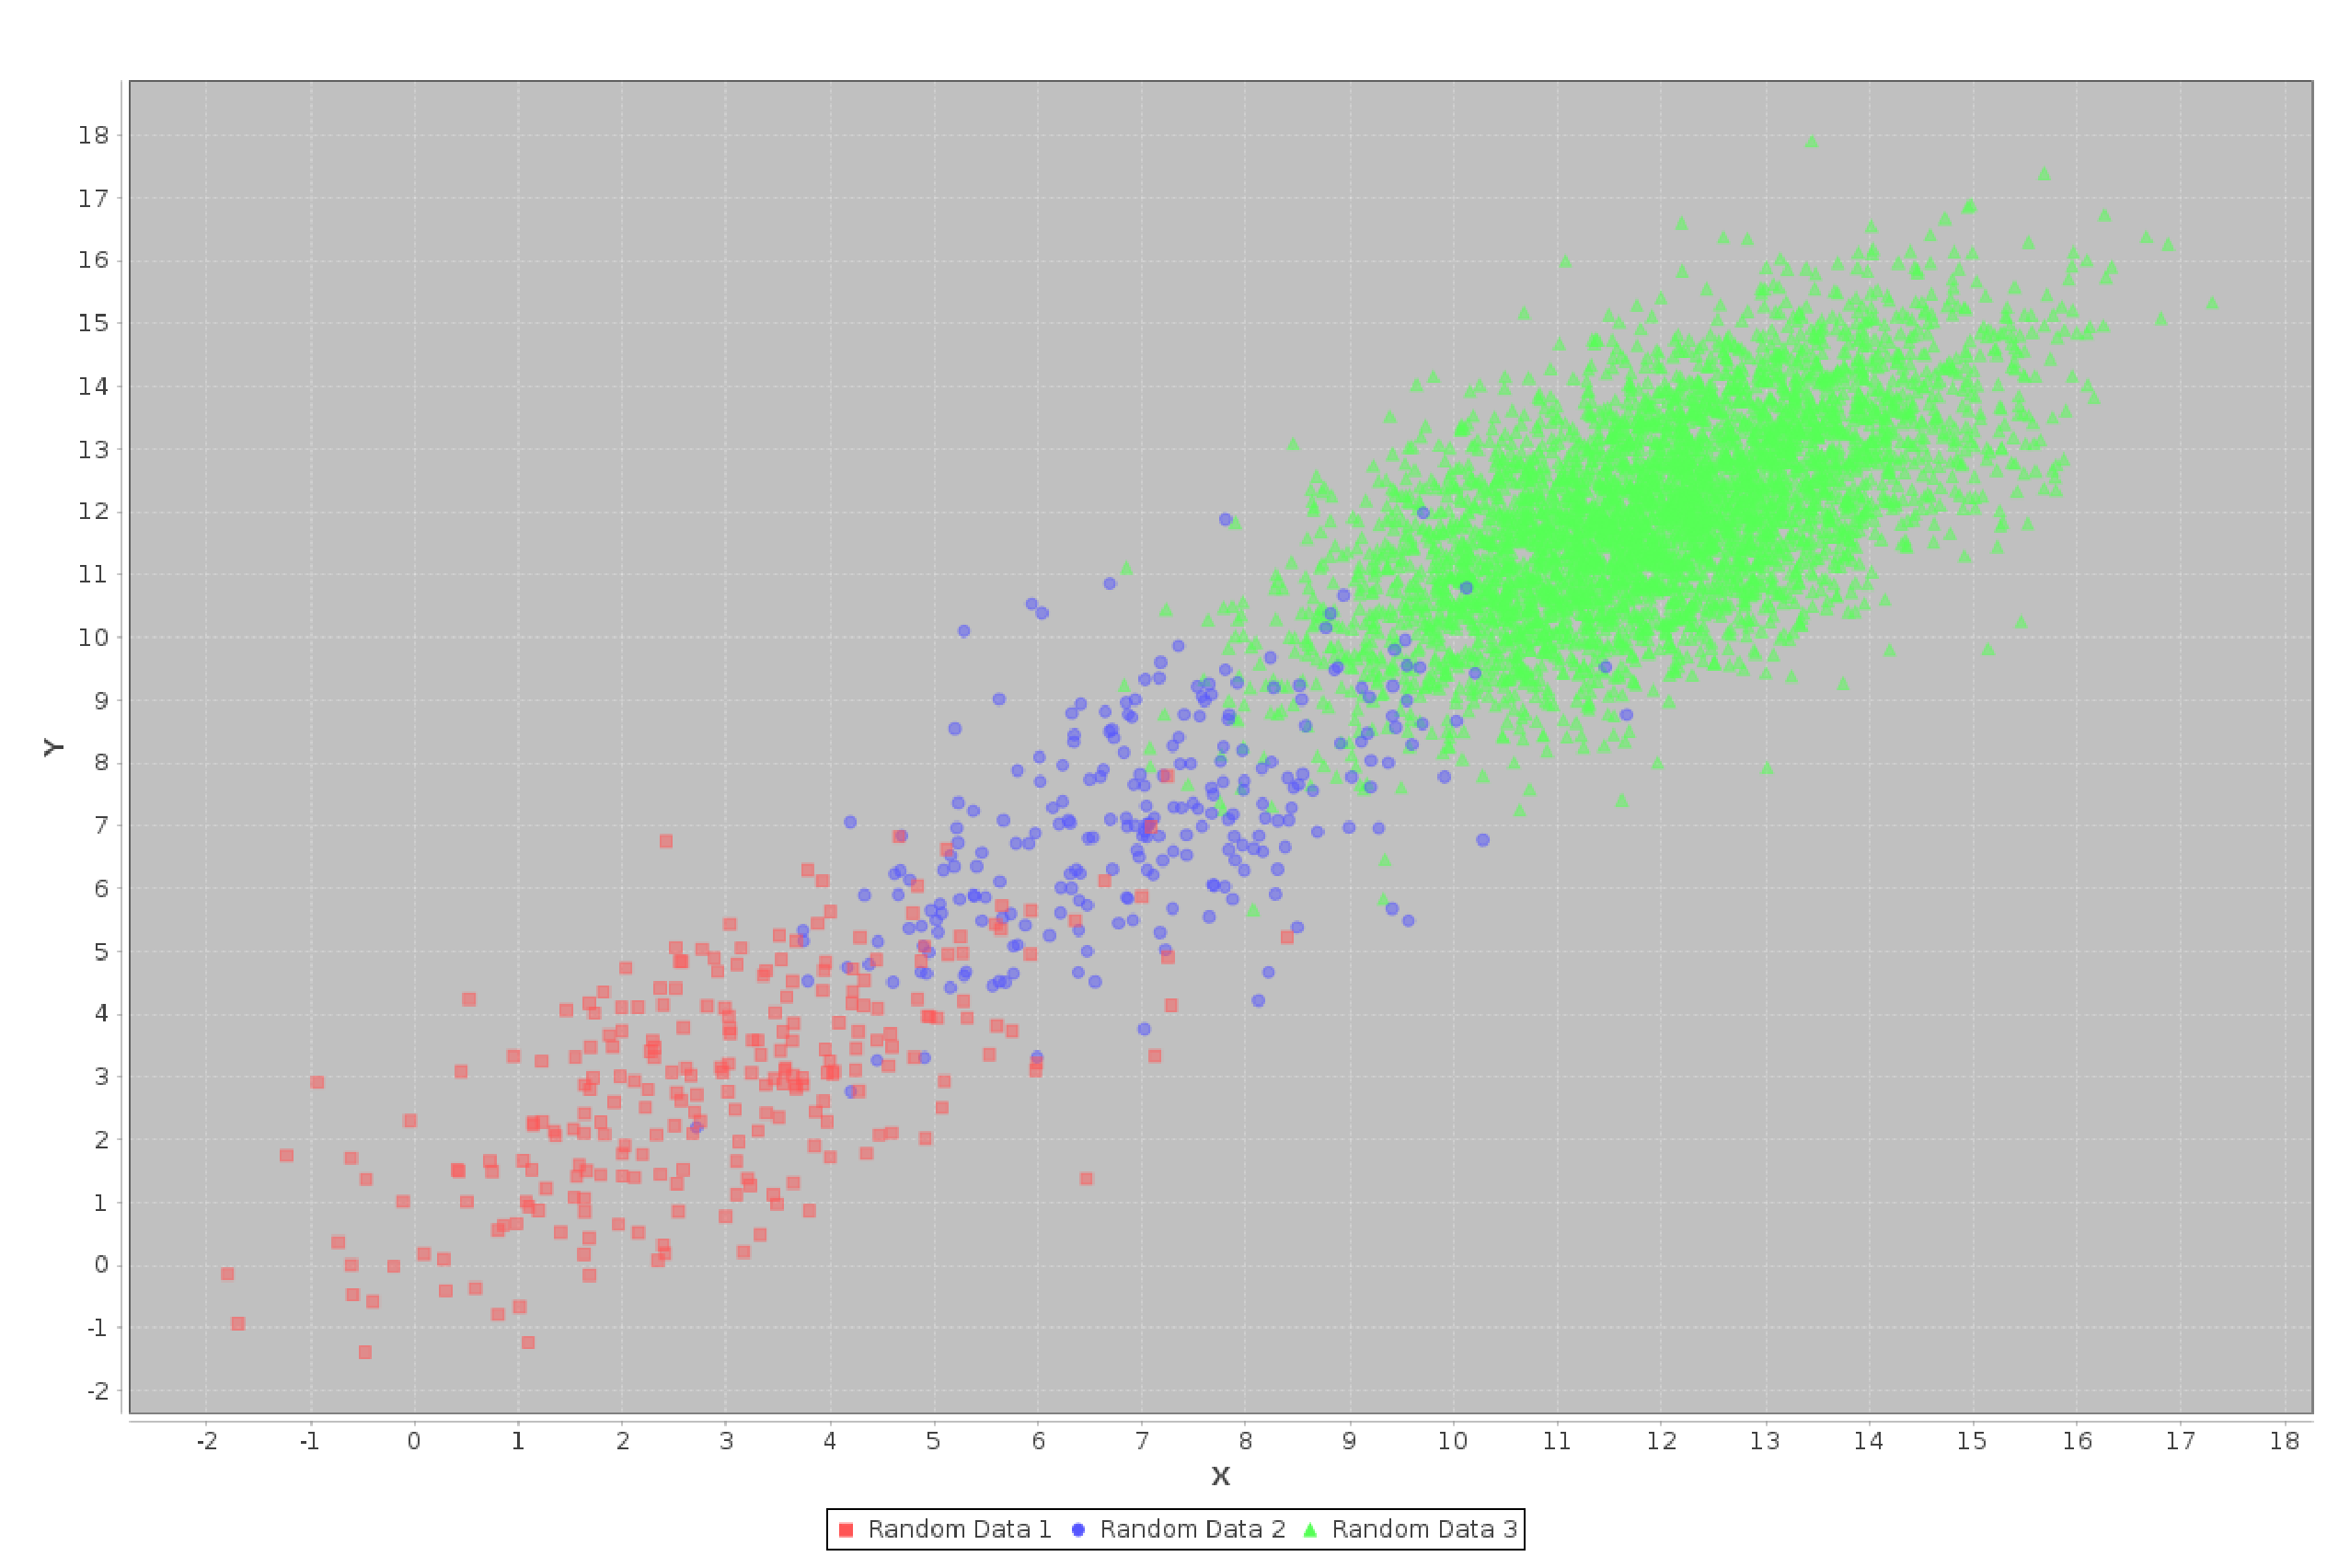
\includegraphics[width=120mm,scale=0.7]{images/dist250-4000-12.eps}
  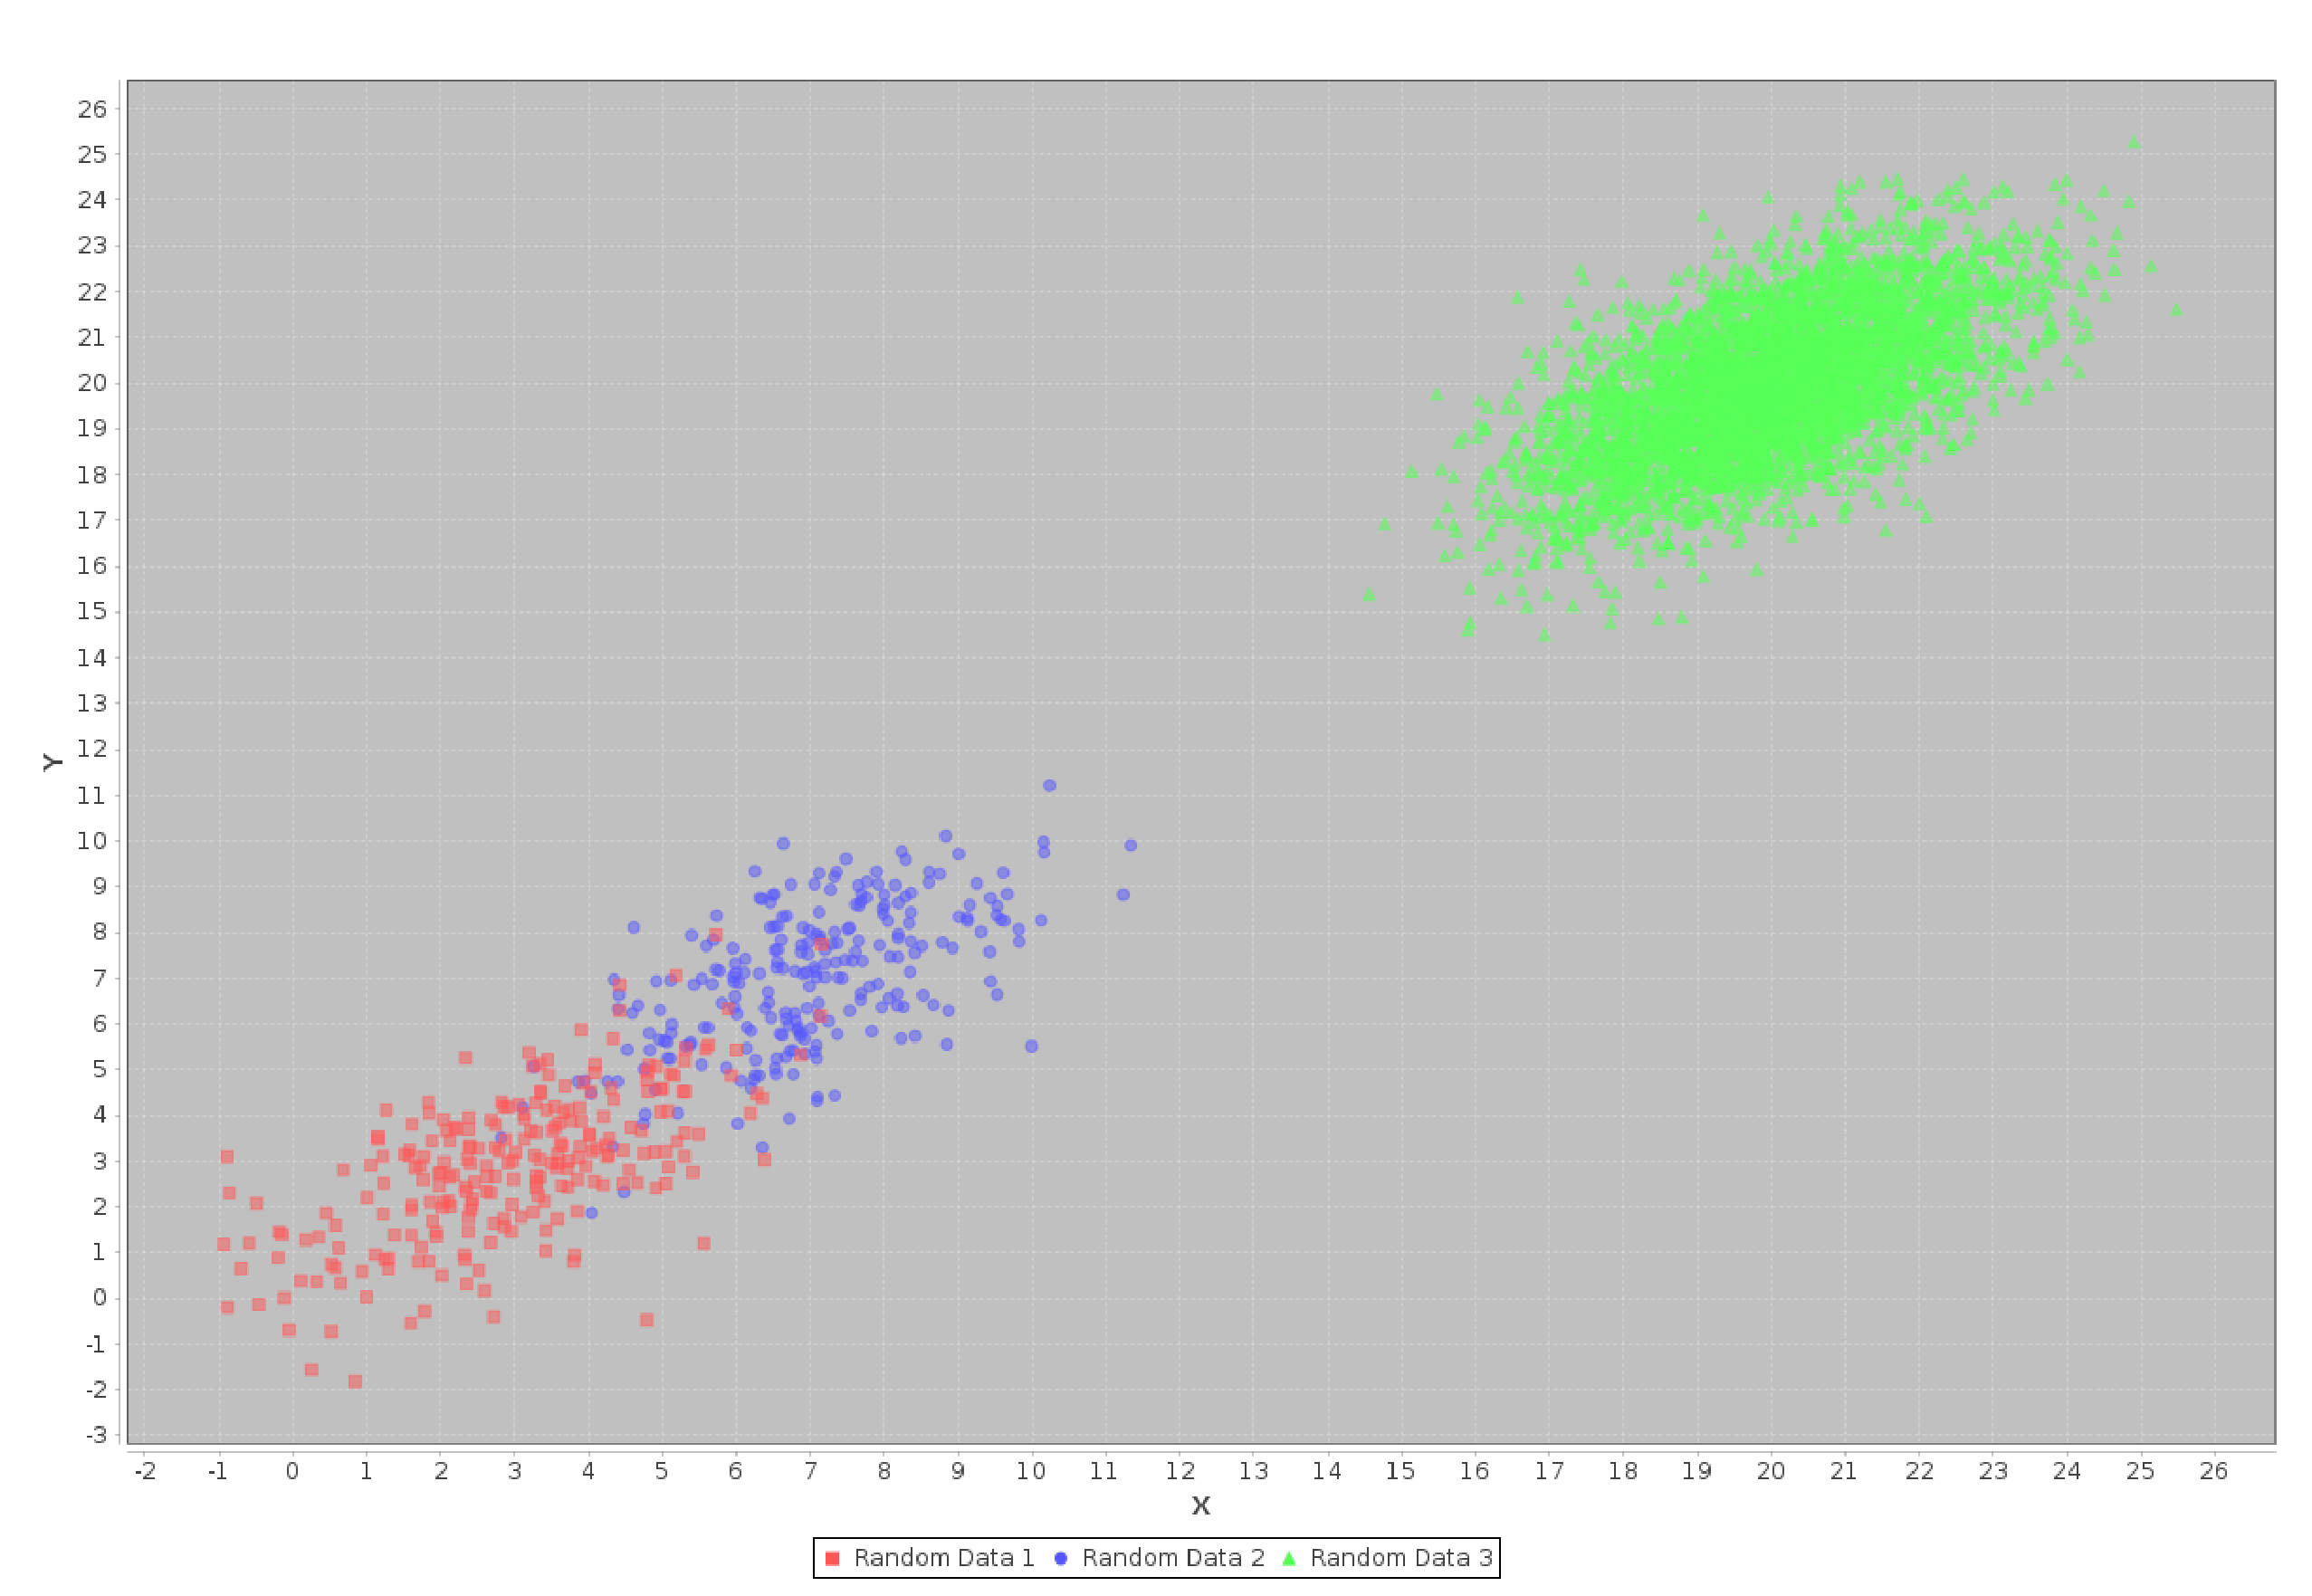
\includegraphics[width=120mm,scale=0.7]{images/dist250-4000-20.eps}
  \caption{Conjuntos de dados sintéticos com a média da distribuição da classe dominante (verde) deslocada}
  \label{fig:dist_iguais}
\end{figure}

\subsection{Resultados dos Testes com os Dados Sintéticos}

Utilizamos nove conjuntos de dados sintéticos diferentes nos testes apresentados nesta seção.
Cada conjunto combina a característica \textit{balanceado}, \textit{normal} ou \textit{ desbalanceado} com uma das configurações de posições de distribuições de classe \textit{próxima}, \textit{adjacente} ou \textit{distante}.
Com isso pudemos testar o comportamento do método de duas formas.
Na primeira verificamos como o método reage à variações no balanceamento entre classes.
Na segunda estudamos a influência da posição das distribuições de classes, i.e. elas podem estar sobrepostas, ter apenas uma interseção parcial ou serem totalmente disjuntas.

Para medir os resultados utilizamos as mesmas métricas \textit{k-Acurácia}, \textit{k-Precision} e \textit{k-Recall} apresentadas anteriormente.
Lembre que essas duas últimas vem em três tipos \textit{Micro}, \textit{Ponderada} (média ponderada das classes) e \textit{Macro} (média aritmética das classes).

Separamos na Tabela \ref{tab:ganho_meta} alguns dos resultados de destaque encontrados durante os experimentos com dados sintéticos.
É importante notar que os números apresentados nesta tabela são as diferenças entre os resultados do metaclassificador e do classificador simples.
Portanto um resultado positivo significa que o método superou o \textit{benchmark} por um percentual com aquele valor.

Como vimos anteriormente o \textit{Micro Precision} e o \textit{Micro Recall} sempre são iguais.
Além disso, o \textit{Precision Ponderado} e o \textit{Recall Ponderado} tem valores muito próximos das versões \textit{Micro}.
Portanto não apresentamos todas as métricas na tabela \ref{tab:ganho_meta}, apenas aquelas que foram mais informativas neste teste.

Os resultados apresentados na Tabela \ref{tab:ganho_meta} se referem à testes conduzidos com conjuntos de dados cuja posição das distribuições das classes era \textit{próxima}.
De fato os centros das distribuições de classes nesses conjuntos de dados são \textit{vermelha} = (3,3), \textit{verde} = (5,5) e \textit{azul} = (7,7).
A partir disso, variamos o balanceamento entre as classes ao longo do teste.
A Tabela \ref{tab:ganho_meta} identifica se os dados são balanceados (B), normais (N) ou desbalanceados (D), conforme foi detalhado na seção \ref{sub:descsinteticos}.

\begin{table}[h!]
  \begin{center}
   \resizebox{\textwidth}{!} {
   \begin{tabular}{cccccc}
      \hline
      \textbf{Algoritmo} & \textbf{Dados} &  \textbf{2-Acu.} & \textbf{2-Prec./Rec.} & \textbf{2-Prec.} & \textbf{2-Rec.} \\
          &     &     & \textbf{(Micro)} & \textbf{(Macro)} & \textbf{(Macro)} \\
      \hline


Árvore	&	B	&	0.24	&	0.33	&	0.32	&	0.33	\\
Árvore	&	N	&	0.99	&	0.98	&	1.45	&	1.45	\\
Árvore	&	D	&	1.04	&	1.04	&	6.8	&	6.27	\\
KNN 5	&	B	&	3.46	&	8	&	7.92	&	8	\\
KNN 5	&	N	&	2.78	&	4.27	&	5.41	&	4.4	\\
KNN 5	&	D	&	1.69	&	1.73	&	7.06	&	9.9	\\
KNN 7	&	B	&	7.32	&	10.58	&	8.53	&	9.01	\\
KNN 7	&	N	&	-0.41	&	-0.67	&	-0.97	&	-0.78	\\
KNN 7	&	D	&	-0.38	&	0	&	0	&	0	\\
KNN 9	&	B	&	1.64	&	4.29	&	4.29	&	4.29	\\
KNN 9	&	N	&	1.12	&	2	&	2.48	&	2.58	\\
KNN 9	&	D	&	1.04	&	1	&	4.61	&	5.88	\\
R. Forest	&	B	&	0.99	&	1.64	&	1.64	&	1.64	\\
R. Forest	&	N	&	0.53	&	0.84	&	1	&	1.09	\\
R. Forest	&	D	&	0.67	&	0.62	&	3.37	&	3.61	\\

      \hline
    \end{tabular}
    }
    \caption{Valores percentuais de ganho do Metaclassificador em relação ao \textit{Benchmark}}
    \label{tab:ganho_meta}
  \end{center}
\end{table}

É possível observar na Tabela \ref{tab:ganho_meta} que o algoritmo \textit{Árvore de Decisão } ganha por uma margem maior que 6\% no \textit{2-Precision Macro} e no \textit{2-Recall Macro} quando os dados são \textit{desbalanceados}.
Em contraste, neste mesmo cenário, o ganho é de apenas 1\% para as métricas \textit{2-Acurácia}, \textit{2-Precision Micro} e \textit{2-Recall Micro}.

Note entretanto que essas últimas métricas não tratam todas as classes do conjunto de dados por igual.
A Acurácia é uma medida geral do desempenho do modelo que simplesmente avalia a quantidade de instâncias corretamente classificadas.
Enquanto a versão \textit{Micro} do \textit{Precision} e \textit{Recall} contabilizam os totais de \textit{true positives}, \textit{false positives} e \textit{false negatives} para a partir destes calcularem os valores finais.
Desta forma, uma classe dominante com maior quantidade de instâncias, como é o caso da classe \tectit{verde}, tem maior influência no valor final dessas métricas.
Por outro lado, as versões \textit{Macro} do \textit{Precision} e \textit{Recall} são uma \textit{média aritmética} das métricas de cada classe.
Portanto, em um cenário com dados desbalanceados, essas últimas tem a sensibilidade para capturar de forma mais evidente as variações de desempenho do modelo para todas as classes do conjunto de dados.

Seguindo com a mesma análise das as métricas \textit{Macro Precision} e \textit{Macro Recall}, observamos ganhos em outros algorítimos além das \textit{Árvores de Decisão}.
Para algoritmo \textit{KNN 5} os ganhos foram de aproximadamente 7\% e 10\%, para o \textit{KNN 9} de 4,5\% e 6\% e para o \textit{Random Forest} de 3,5\%.
Desta forma podemos concluir que o método proposto foi eficiente para melhorar o resultado desses algorítimos em um cenário com dados desbalanceados e com distribuições de classes muito próximas.

Outro conjunto notável de resultados que podem ser vistos na Tabela \ref{tab:ganho_meta} são aqueles referentes aos dados perfeitamente balanceados.
Note que neste contexto o algoritmo \textit{KNN 5} exibe ganhos de cerca de 8\% em todas as métricas \textit{Precision} e \textit{Recall}.
Um ganho de desempenho similar, embora menor, pode ser visto nos testes com os algoritmos \textit{KNN 9} e \textit{Random Forest}.
Este cenário de testes é especial pois representa uma tarefa mais difícil para muitos algoritmos.
Lembre que neste caso as médias das distribuições das três classes do conjunto de dados estão muito próximas e portanto estas tem uma grande interseção no espaço amostral (vide primeira imagem da Figura \ref{fig:dist_diferentes}).
Este resultado demonstra que o método proposto também melhorou o desempenho desses algoritmos neste caso.

Por fim, ainda é possível observar ganhos de 3,5\% a 5,5\% no \textit{Precision} e \textit{Recall} para o algoritmo \textit{KNN 5} nos testes com dados do tipo \textit{normal}.
Recorde que estes são um meio termo entre os dados \textit{balanceados} e \textit{desbalanceados}.
Ganhos menores são observáveis na mesma situação para os algorítimos \textit{KNN 9} e \textit{Random Forest}.
Novamente este resultado reforça que o método proposto melhora o resultado desses algoritmos para conjuntos de dados cujas classes tem distribuições com médias muito próximas e que portanto se sobrepõem.

Como citamos, diversos outros testes com dados sintéticos foram feitos mas mostramos apenas os resultados de interesse nesta seção.
Realizamos os mesmos testes discutidos aqui com dados onde as distribuições das classes estão mais afastadas (\textit{adjacente} e \textit{distante}), conforme ilustrado na Figura \ref{fig:dist_iguais}.
Porém nestes demais cenários o metaclassificador não se destacou de maneira substancial.
Embora ele tenha apresentado algum ganho na maioria dos casos, estes são iguais ou inferiores a 1\%.
Para ver o restante dos resultados com os dados sintéticos consulte o apêndice desta dissertação.
